\chapter{Eccodes for Grib, Opendata, NetCDF, Visualization}

Meteorological data are often stored in GRIB or NetCDF formats, both of which are compact binary formats widely used in numerical weather prediction and climate analysis. While GRIB is the standard format for meteorological model outputs, NetCDF is more commonly used in the broader scientific community, particularly for observational datasets and climate research. Additionally, Zarr is an alternative format to NetCDF, optimized for cloud-based storage and parallel computing for machine learning applications. Recent developments allow storing NetCDF data in Zarr format for enhanced scalability.

In this chapter, we demonstrate how to work with both formats, focusing on GRIB data using the ECCODES library---provided by ECMWF---to decode and analyze meteorological data from the {\em DWD Open Data Server}, and working with NetCDF for further integration and analysis. We will cover the following steps:

\begin{itemize}
    \item {\em Accessing and Downloading GRIB Data}: Retrieving ICON model GRIB files, including latitude-longitude fields and the 2-m temperature field, from the DWD Open Data Server.
    \item {\em Inspecting GRIB File Metadata}: Listing GRIB file keys, understanding metadata, and summarizing the available parameters and levels.
    \item {\em Loading and Visualizing GRIB Data}: Extracting numerical fields, mapping the spatial coordinates, and plotting meteorological variables using visualization tools.
\end{itemize}

In addition, we introduce NetCDF as a fundamental format for meteorological and climate data, covering the following aspects:

\begin{itemize}
    \item {\em Accessing and Managing NetCDF Data}: Understanding the structure of NetCDF files, reading data, and managing metadata.
    \item {\em Working with NetCDF Data}: Processing and analyzing NetCDF datasets in the context of meteorological applications.
    \item {\em Visualizing NetCDF Data}: Plotting and interpreting NetCDF data using scientific computing tools.
\end{itemize}

By following these steps, we will gain a complete workflow for handling ICON model GRIB and NetCDF files, from downloading and inspection to visualization and analysis for scientific applications.


%==============================================================================
%
%==============================================================================
\section{Downloading ICON Model GRIB Files from DWD Open Data Server}

To analyze meteorological data using the ICON model, we need to download the required GRIB files from the \emph{DWD Open Data Server}. These include the \emph{2-meter temperature field} (\texttt{icon\_t2m.grib}), the \emph{latitude grid} (\texttt{icon\_lat.grib}), and the \emph{longitude grid} (\texttt{icon\_lon.grib}). DWD provides these files in compressed GRIB2 format (\texttt{.grib2.bz2}), which must be downloaded and extracted before further processing. 

{\bf Downloading the 2-Meter Temperature Field.} 

The following script constructs the filename for the \emph{latest 2m temperature GRIB file} based on the current UTC date, downloads it using \texttt{wget}, and extracts it.

\begin{codeonly}{Downloading 2m Temperature Data}
import datetime
import os
import wget
import bz2

# Construct the filename based on the current UTC date
now = datetime.datetime.now(datetime.UTC)
filename = f"icon_global_icosahedral_single-level_{now:%Y%m%d}00_000_T_2M.grib2.bz2"
print("Constructed filename:", filename)

# Define the base URL
base_url = "https://opendata.dwd.de/weather/nwp/icon/grib/00/t_2m/"
url = base_url + filename
print("Download URL:", url)

# Download the .bz2 file using Python wget
wget.download(url, filename)
print(f"\nDownloaded {filename}")

# Decompress the .bz2 file using bz2 module
with bz2.open(filename, 'rb') as f_in, open(filename[:-4], 'wb') as f_out:
    f_out.write(f_in.read())
print(f"Decompressed {filename} to {filename[:-4]}")

# Rename to a standard name
grib_filename = filename[:-4]
final_filename = "icon_t2m.grib"
os.rename(grib_filename, final_filename)
print(f"Renamed {grib_filename} to {final_filename}")
\end{codeonly}

This script ensures that the latest available \emph{2m temperature} field will be automatically retrieved and prepared for use.

{\bf Downloading Latitude and Longitude Data.} 

The latitude (\texttt{icon\_lat.grib}) and longitude (\texttt{icon\_lon.grib}) grids are \emph{time-invariant} and must be downloaded separately. The script below identifies the latest available version on the DWD server, downloads both files, and renames them for easier access. The following script is contained in the file \texttt{icon\_grid\_get.py} as well as in the jupyter notebook to catch forecasts from the DWD open data server. 

\begin{codeonly}{Downloading ICON Latitude and Longitude GRIB Data}
import re
import os
import bz2
import requests
import wget

base_url = "https://opendata.dwd.de/weather/nwp/icon/grib/00/"
clat_path = "clat/"
clon_path = "clon/"

# Function to find the latest available timestamp from DWD server
def get_latest_timestamp(path):
    listing_url = base_url + path
    response = requests.get(listing_url)
    if response.status_code != 200:
        raise RuntimeError(f"Could not fetch listing: {listing_url}")
    timestamps = re.findall(
        r'icon_global_icosahedral_time-invariant_(\d{10})_CLAT\.grib2\.bz2',
        response.text
    )
    return max(timestamps) if timestamps else None

# Get the latest available timestamp
timestamp = get_latest_timestamp(clat_path)
if not timestamp:
    raise RuntimeError("Could not determine latest timestamp from DWD server.")

files = {
    "clat": f"clat/icon_global_icosahedral_time-invariant_{timestamp}_CLAT.grib2.bz2",
    "clon": f"clon/icon_global_icosahedral_time-invariant_{timestamp}_CLON.grib2.bz2"
}

rename_map = {"clat": "icon_lat.grib", "clon": "icon_lon.grib"}

for key, path in files.items():
    filename = os.path.basename(path)
    url = base_url + path

    print(f"Downloading {url} ...")
    wget.download(url, filename)
    print(f"\nDownloaded {filename}")

    # Uncompress the .bz2 file
    with bz2.open(filename, 'rb') as compressed, open(filename[:-4], 'wb') as out_file:
        out_file.write(compressed.read())
    print(f"Decompressed {filename} to {filename[:-4]}")

    # Rename the extracted file
    extracted_filename = filename[:-4]  # Remove .bz2
    new_filename = rename_map[key]
    os.rename(extracted_filename, new_filename)
    print(f"Renamed {extracted_filename} to {new_filename}")
\end{codeonly}

This script identifies the \emph{latest available latitude and longitude files} on the DWD server, downloads them using \texttt{wget}, extracts the \texttt{.bz2} compressed files, and renames them to \texttt{icon\_lat.grib} and \texttt{icon\_lon.grib} for easy reference.

After executing these scripts, we have all necessary \emph{spatial coordinate data and temperature fields} to proceed with further analysis and visualization.


%==============================================================================
%
%==============================================================================
\section{The Grib Library eccodes}

We have discussed the download of grib data, here we now assume that we have icon lat and lon coordinates in files \texttt{icon\_lat.grib} and  \texttt{icon\_lon.grib}. 

\texttt{ecCodes} is a library developed by ECMWF for decoding and encoding GRIB (GRIdded Binary) files. It provides a Python interface to inspect and manipulate meteorological data stored in the GRIB format.

{\bf Installing ecCodes.} Installing \texttt{ecCodes}, the ECMWF library for GRIB file handling, can be challenging due to dependencies and system configurations. Here is a summary of the installation process:

{\bf System Dependencies}: Ensure required system libraries are installed:
\begin{lstlisting}
sudo apt update && sudo apt install libeccodes-dev eccodes
\end{lstlisting}
On macOS, use Homebrew:
\begin{lstlisting}
brew install eccodes
\end{lstlisting}

{\bf Python Package}: Install the Python bindings with:
\begin{verbatim}
pip install eccodes
\end{verbatim}

\begin{recommendationbox}
Using ECCODES on Windows should be done via windows subsystem for linux or through a docker container. 
\end{recommendationbox}

On Windows, you should use the {\bf WSL} (Windows Subsystem for Linux). Here, you can do the same install commands
\begin{lstlisting}
sudo apt update
sudo apt install eccodes
sudo apt install libeccodes-tools
\end{lstlisting}

Test it with 
\begin{lstlisting}
grib_ls -V
\end{lstlisting}

{\bf Setting Environment Variables}: If the library is not found, define the paths manually:
\begin{lstlisting}
export ECCODES_DEFINITION_PATH=/usr/share/eccodes/definitions
export ECCODES_SAMPLES_PATH=/usr/share/eccodes/samples
\end{lstlisting}
Adjust these paths according to your system setup.

{\bf Verifying Installation}: Check if ecCodes is working correctly:
\begin{lstlisting}
grib_ls --help
python -c "import eccodes; print(eccodes.codes_get_api_version())"\end{lstlisting}
If these commands return valid output, the installation is successful.

{\bf Handling DWD-Specific Definitions}: If working with DWD GRIB files, additional definition files may be required. Download the latest version from:
\begin{lstlisting}
https://opendata.dwd.de/weather/lib/grib/
\end{lstlisting}
We provide a script \texttt{download\_latest\_grib\_definition\_dwd.py} which will carry out the download and installation, but still needs you to take care of the path variables. 
Please check and make sure the definitions paths are set properly. 


{\bf Checking if ecCodes is Installed}
Before using \texttt{ecCodes}, you can check if it is installed correctly with the following code:

\begin{codeonly}{Checking ecCodes Installation}
try:
    import eccodes
    print("ecCodes is installed and working correctly.")
except ImportError:
    print("ecCodes is not installed. Please install it using 'pip install eccodes'.")
    exit(1)
\end{codeonly}


{\bf Inspecting Grib Files.}
We next demonstrate how to inspect the metadata keys and shortnames of GRIB files (\texttt{icon\_lat.grib} and \texttt{icon\_lon.grib}) using \texttt{ecCodes}.

{\bf Listing GRIB Keys.} The function below extracts and lists metadata keys from a GRIB file:

\begin{codeonly}{Listing GRIB Keys}
import eccodes

def list_grib_keys(grib_filename):
    """Lists keys from a GRIB file while handling errors properly."""
    try:
        with open(grib_filename, 'rb') as f:
            while True:
                gid = eccodes.codes_grib_new_from_file(f)
                if gid is None:  # End of file
                    break

                key_iterator = eccodes.codes_keys_iterator_new(gid)
                keys = []

                while eccodes.codes_keys_iterator_next(key_iterator):
                    keyname = eccodes.codes_keys_iterator_get_name(key_iterator)
                    if keyname not in ['section2Padding', 'codedValues', 'values']:
                        try:
                            value = eccodes.codes_get_string(gid, keyname)
                        except Exception:
                            value = "N/A"
                        keys.append((keyname, value))

                eccodes.codes_release(gid)
                
                # Print all extracted keys
                for key, value in keys:
                    print(f"Key: {key:40} Value: {value}")
    except eccodes.CodesInternalError as e:
        print(f"ecCodes Error: {e}")

# Example usage
list_grib_keys("icon_lat.grib")
\end{codeonly}

Output can be e.g.\
\begin{codeonly}{Keys}
Key: globalDomain                             Value: g
Key: GRIBEditionNumber                        Value: 2
Key: tablesVersionLatestOfficial              Value: 32
Key: tablesVersionLatest                      Value: 32
Key: grib2divider                             Value: 1e+06
Key: angleSubdivisions                        Value: 1e+06
Key: missingValue                             Value: 9999
Key: ieeeFloats                               Value: 1
Key: isHindcast                               Value: 0
...
\end{codeonly}


{\bf Listing Short Names from a GRIB File.}

The function below extracts and lists short names along with their corresponding levels and sizes from a GRIB file:

\begin{codeonly}{Listing Short Names}
import eccodes

def show_shortnames(grib_file):
    """Lists short names, levels, and sizes from a GRIB file."""
    with open(grib_file, 'rb') as f:
        shortName_prev = ''
        output = ''
        level_prev = ''
        count = 0
        print('-' * 80)
        print('File = ', grib_file)
        print('\n{:<30}{:<16}{:>10}'.format('Short Name', 'Level', 'Size'))
        print('-' * 80)
        while True:
            gid = eccodes.codes_grib_new_from_file(f)
            if gid is None:
                break
            shortName = eccodes.codes_get(gid, "shortName")
            level = eccodes.codes_get(gid, "level")
            size1 = eccodes.codes_get_size(gid, "values")
            if shortName_prev != shortName:
                if level_prev != level and count > 0:
                    output += f' - {level_prev}'
                if count > 0:
                    output += f', \t Size = {size1}'
                output += '\n{:<30}{:<16}{:>10}'.format(shortName, level, size1)
                shortName_prev = shortName
                level_prev = level
                count += 1
            eccodes.codes_release(gid)
        print(output)

# Example usage
show_shortnames("icon_lat.grib")
\end{codeonly}

Output is something like e.g.\

\begin{codeonly}{Shortnames, Levels, Size}
--------------------------------------------------------------------------------
File =  icon_lat.grib
Short Name                    Level                 Size
--------------------------------------------------------------------------------
tlat                          0                  2949120
\end{codeonly}

These functions allow users to inspect the GRIB file structure, understand available variables, and extract key metadata for further analysis.

{\bf Plotting Latitude and Longitude Data.} To visualize the points stored in the GRIB files, we use \texttt{matplotlib} along with \texttt{cartopy} to overlay the scatter plot on a map:

\begin{codeonly}{Plotting Latitude and Longitude with a Map}
import eccodes
import numpy as np
import matplotlib.pyplot as plt
import cartopy.crs as ccrs
import cartopy.feature as cfeature

def plot_lat_lon(lat_file, lon_file):
    """Plots latitude and longitude points from GRIB files on a map."""
    def extract_values(grib_file):
        with open(grib_file, 'rb') as f:
            gid = eccodes.codes_grib_new_from_file(f)
            values = eccodes.codes_get_array(gid, "values")
            eccodes.codes_release(gid)
        return values
    
    latitudes = extract_values(lat_file)
    longitudes = extract_values(lon_file)
    
    plt.figure(figsize=(10, 5))
    ax = plt.axes(projection=ccrs.PlateCarree())
    ax.set_global()
    ax.add_feature(cfeature.LAND, edgecolor='black')
    ax.add_feature(cfeature.COASTLINE)
    ax.add_feature(cfeature.BORDERS, linestyle=':')
    
    plt.scatter(longitudes, latitudes, s=0.5, color='gray', transform=ccrs.PlateCarree())
    plt.xlabel("Longitude")
    plt.ylabel("Latitude")
    plt.title("Scatter Plot of Latitude and Longitude on a Map")
    plt.grid()
    plt.savefig("icon_points_global.png", dpi=300, bbox_inches='tight')
    plt.show()

# Example usage
plot_lat_lon("icon_lat.grib", "icon_lon.grib")
\end{codeonly}

This function:
\begin{itemize}
    \item Reads latitude and longitude values from GRIB files.
    \item Uses \texttt{matplotlib} and \texttt{cartopy} to overlay the points on a global map.
    \item Adds land, coastlines, and country borders for better visualization.
\end{itemize}

\begin{figure}[ht]
    \centering
    \begin{minipage}{0.5\textwidth}
        \centering
        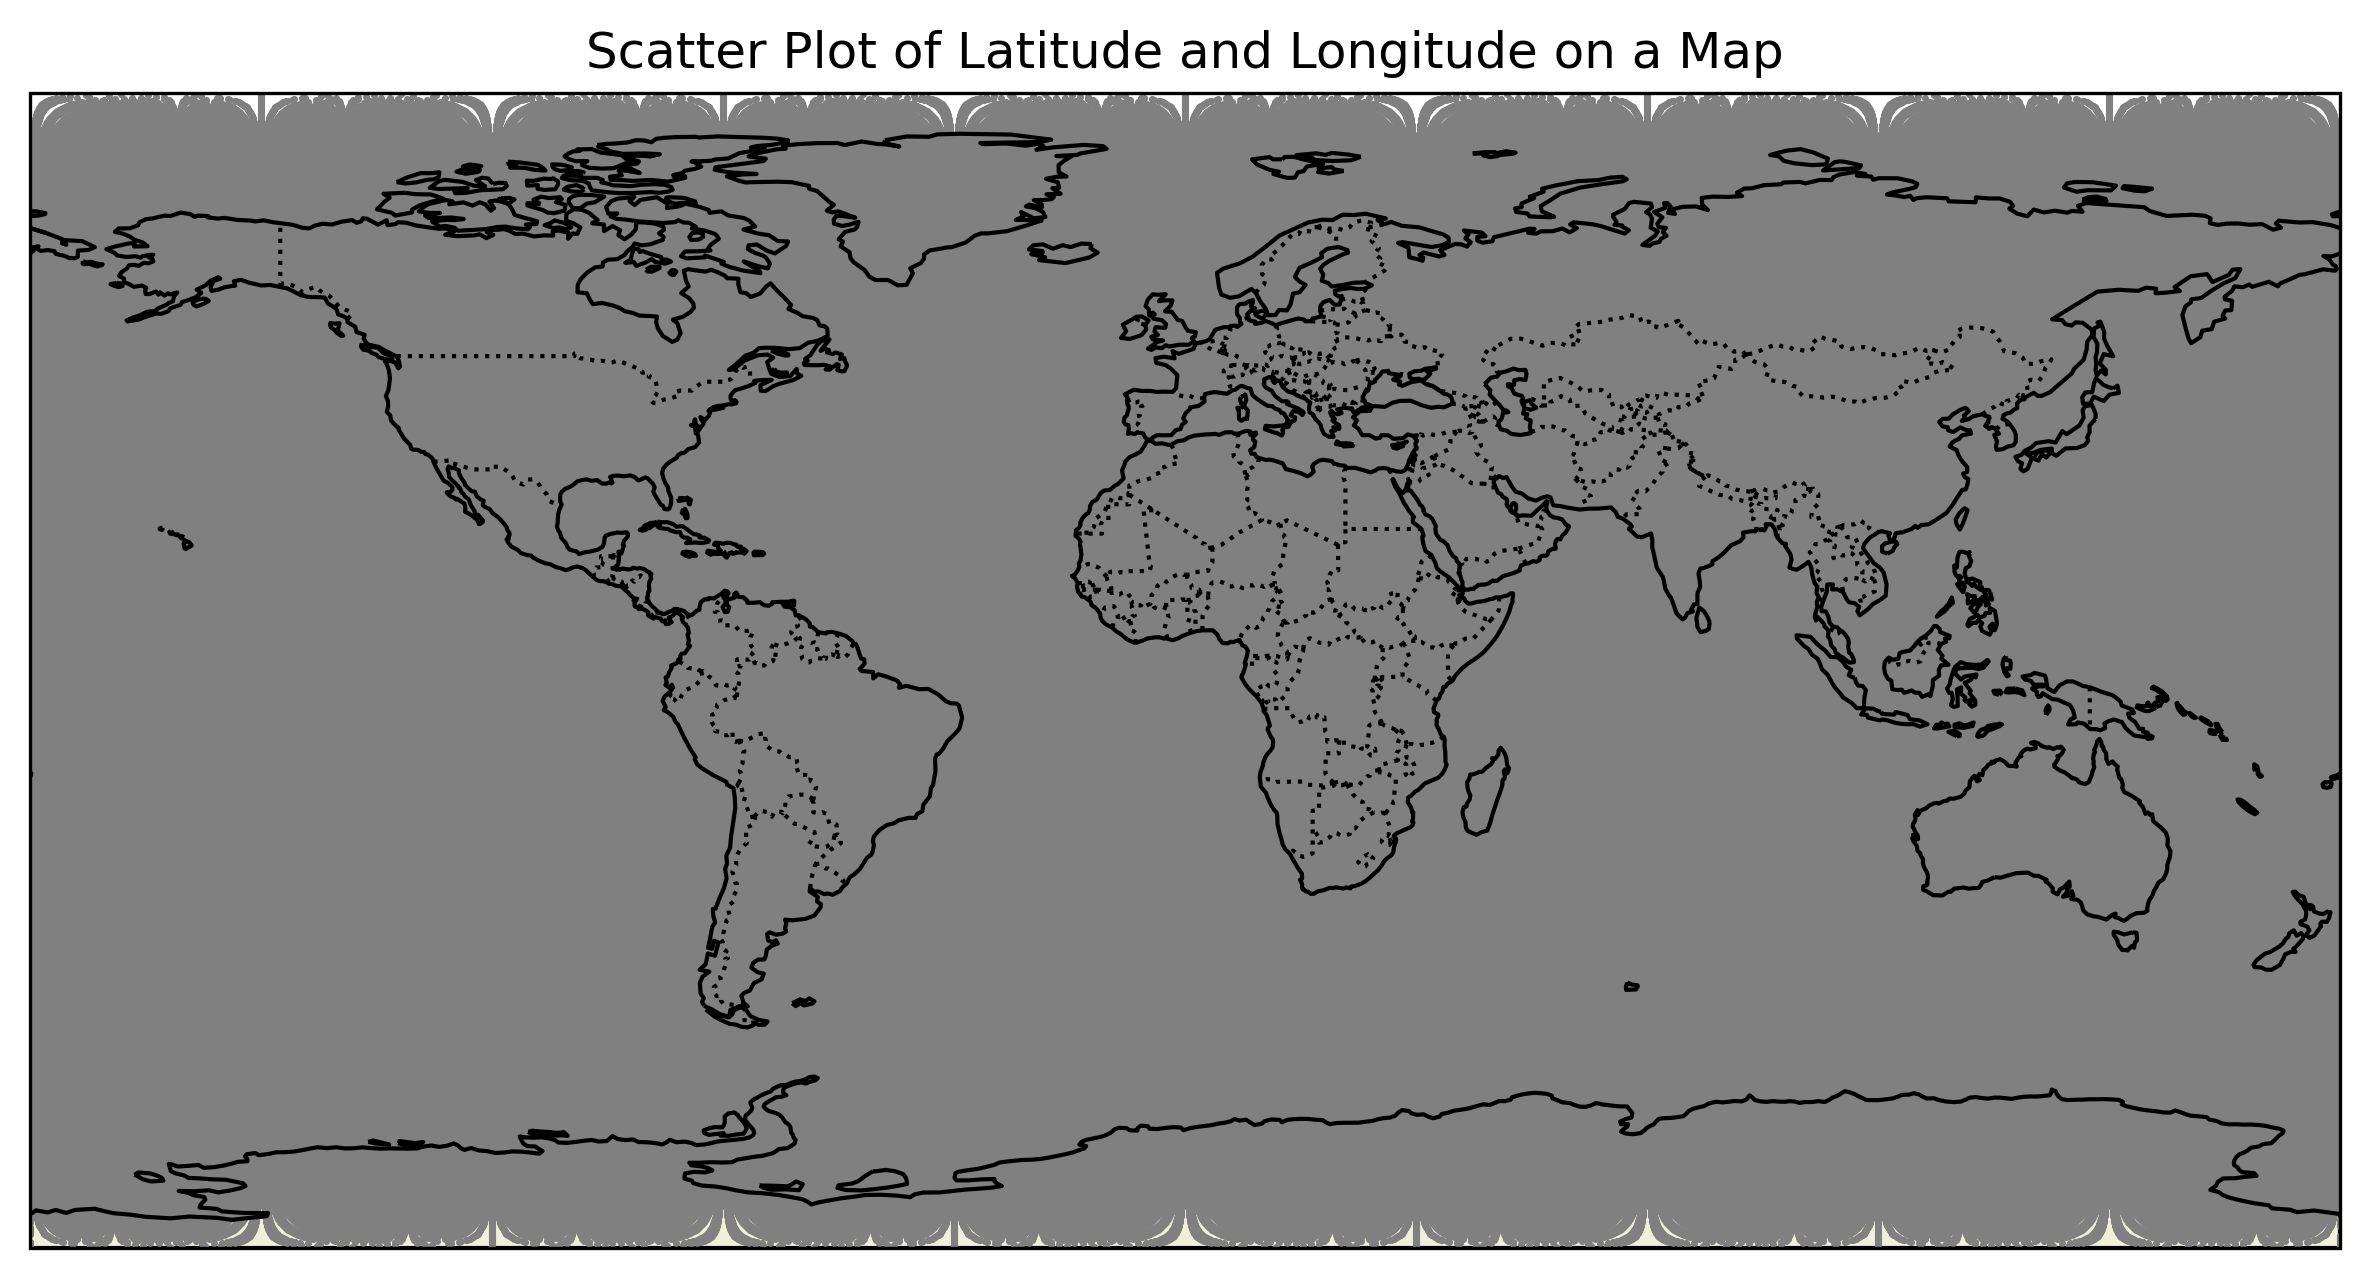
\includegraphics[width=\textwidth]{images/icon_points_global.png}
        \caption{Global ICON grid points.}
        \label{fig:t2m_global_interp}
    \end{minipage}
    \hfill
    \begin{minipage}{0.4\textwidth}
        \centering
        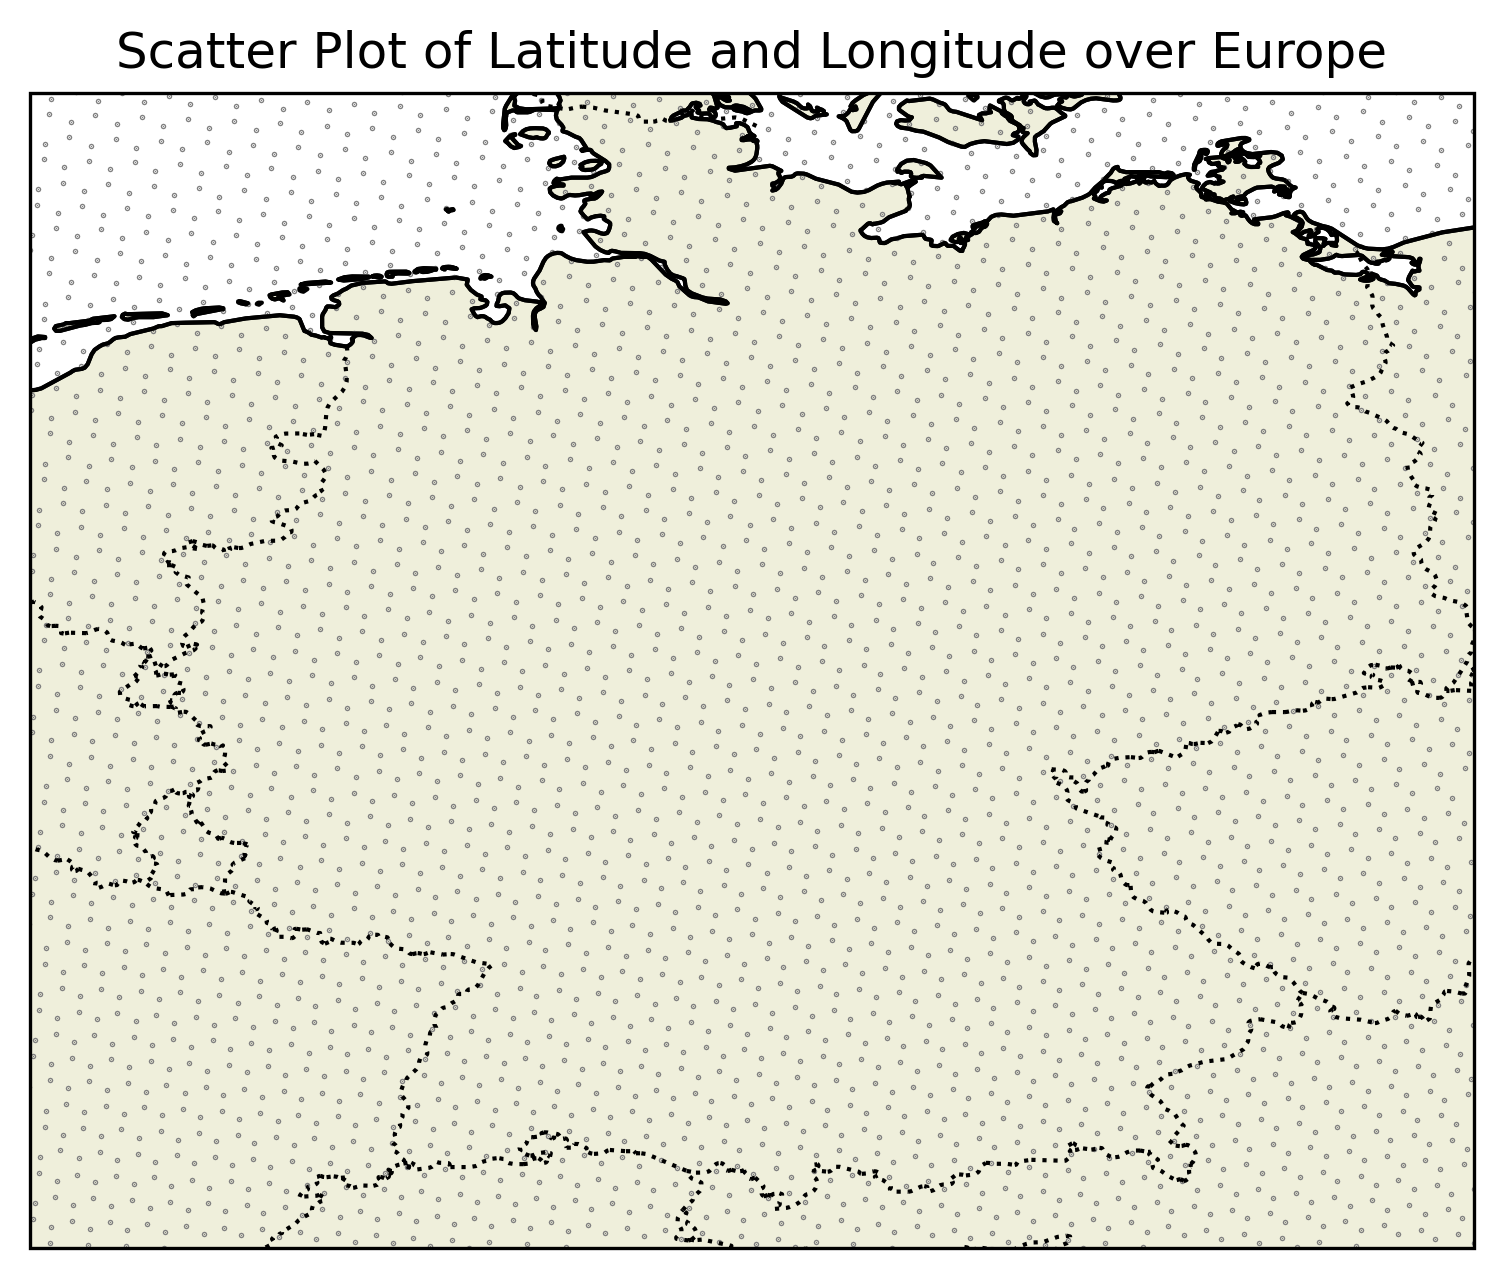
\includegraphics[width=\textwidth]{images/icon_points_germany.png}
        \caption{ICON grid points over Germany.}
        \label{fig:t2m_germany_interp}
    \end{minipage}
\end{figure}

But the resolution is quite high, you cannot see much any more, everything is covered by points. 


{\bf Zooming in Over Germany.} To visualize the points stored in the GRIB files, we use \texttt{matplotlib} along with \texttt{cartopy} to overlay the scatter plot on a map:

\begin{codeonly}{Plotting Latitude and Longitude with a Map}
import eccodes
import numpy as np
import matplotlib.pyplot as plt
import cartopy.crs as ccrs
import cartopy.feature as cfeature

def plot_lat_lon_germany(lat_file, lon_file):
    """Plots latitude and longitude points from GRIB files, zoomed in over Europe."""
    def extract_values(grib_file):
        with open(grib_file, 'rb') as f:
            gid = eccodes.codes_grib_new_from_file(f)
            values = eccodes.codes_get_array(gid, "values")
            eccodes.codes_release(gid)
        return values
    
    latitudes = extract_values(lat_file)
    longitudes = extract_values(lon_file)
    
    plt.figure(figsize=(10, 5))
    ax = plt.axes(projection=ccrs.PlateCarree())
    ax.set_extent([5, 15, 47, 55], crs=ccrs.PlateCarree())  # Europe zoom: [lon_min, lon_max, lat_min, lat_max]
    ax.add_feature(cfeature.LAND, edgecolor='black')
    ax.add_feature(cfeature.COASTLINE)
    ax.add_feature(cfeature.BORDERS, linestyle=':')
    
    plt.scatter(longitudes, latitudes, s=0.1, color='blue', transform=ccrs.PlateCarree())
    plt.xlabel("Longitude")
    plt.ylabel("Latitude")
    plt.title("Scatter Plot of Latitude and Longitude over Europe")
    plt.grid()
    plt.savefig("icon_points_germany.png", dpi=300, bbox_inches='tight')
    plt.show()

# Example usage
plot_lat_lon_germany("icon_lat.grib", "icon_lon.grib")
\end{codeonly}

This function:
\begin{itemize}
    \item Reads latitude and longitude values from GRIB files.
    \item Zooms into Europe with specific latitude/longitude boundaries.
    \item Uses \texttt{matplotlib} and \texttt{cartopy} to overlay the points on a regional map.
    \item Adjusts the point size to avoid excessive density.
\end{itemize}

{\bf Visualizing 2-Meter Temperature (T2M)}

To visualize the 2-meter temperature field from GRIB data, we extract the temperature values alongside the previously loaded latitude and longitude coordinates. The relevant Python function for loading the T2M values is:

\begin{codeonly}{Loading T2M Data}
import eccodes

def load_grib(file, var):
    """Loads specified variable from GRIB file."""
    with open(file, 'rb') as f:
        while (gid := eccodes.codes_grib_new_from_file(f)) is not None:
            if eccodes.codes_get(gid, "shortName") == var:
                vals = eccodes.codes_get_array(gid, "values")
                eccodes.codes_release(gid)
                return vals
            eccodes.codes_release(gid)
    return None

# Load T2M data
t2m = load_grib("icon_t2m.grib", "2t")
\end{codeonly}

Once the temperature values are obtained, they are visualized using \texttt{matplotlib} and \texttt{cartopy}, adapting the point size dynamically based on the bounding box size to maintain clarity across different zoom levels. The visualization function is given below:

\begin{codeonly}{Plotting T2M Data}
import numpy as np
import matplotlib.pyplot as plt
import cartopy.crs as ccrs
import cartopy.feature as cfeature

def plot_t2m(lat, lon, t2m, bbox, title, fname):
    """Plots 2m temperature within bbox = (latmin, latmax, lonmin, lonmax)."""
    latmin, latmax, lonmin, lonmax = bbox
    mask = (lat >= latmin) & (lat <= latmax) & (lon >= lonmin) & (lon <= lonmax)
    
    # Adaptive point size based on bounding box area
    area = (latmax - latmin) * (lonmax - lonmin)
    point_size = max(0.05, min(10, 500 / area))  # Ensures reasonable point size
    
    plt.figure(figsize=(10, 6))
    ax = plt.axes(projection=ccrs.PlateCarree())
    ax.set_extent([lonmin, lonmax, latmin, latmax])
    ax.add_feature(cfeature.LAND, edgecolor='black')
    ax.add_feature(cfeature.COASTLINE)
    ax.add_feature(cfeature.BORDERS, linestyle=':')

    plt.scatter(lon[mask], lat[mask], c=t2m[mask], cmap='jet', s=point_size, transform=ccrs.PlateCarree())
    plt.colorbar(label="Temp (K)")
    plt.title(title)
    plt.savefig(fname, dpi=300, bbox_inches='tight')
    plt.show()
\end{codeonly}

Using this function, we generate two figures displaying the global distribution of 2-meter temperature and a zoomed-in view over Germany.

\begin{figure}[ht]
    \centering
    \begin{minipage}{0.5\textwidth}
        \centering
        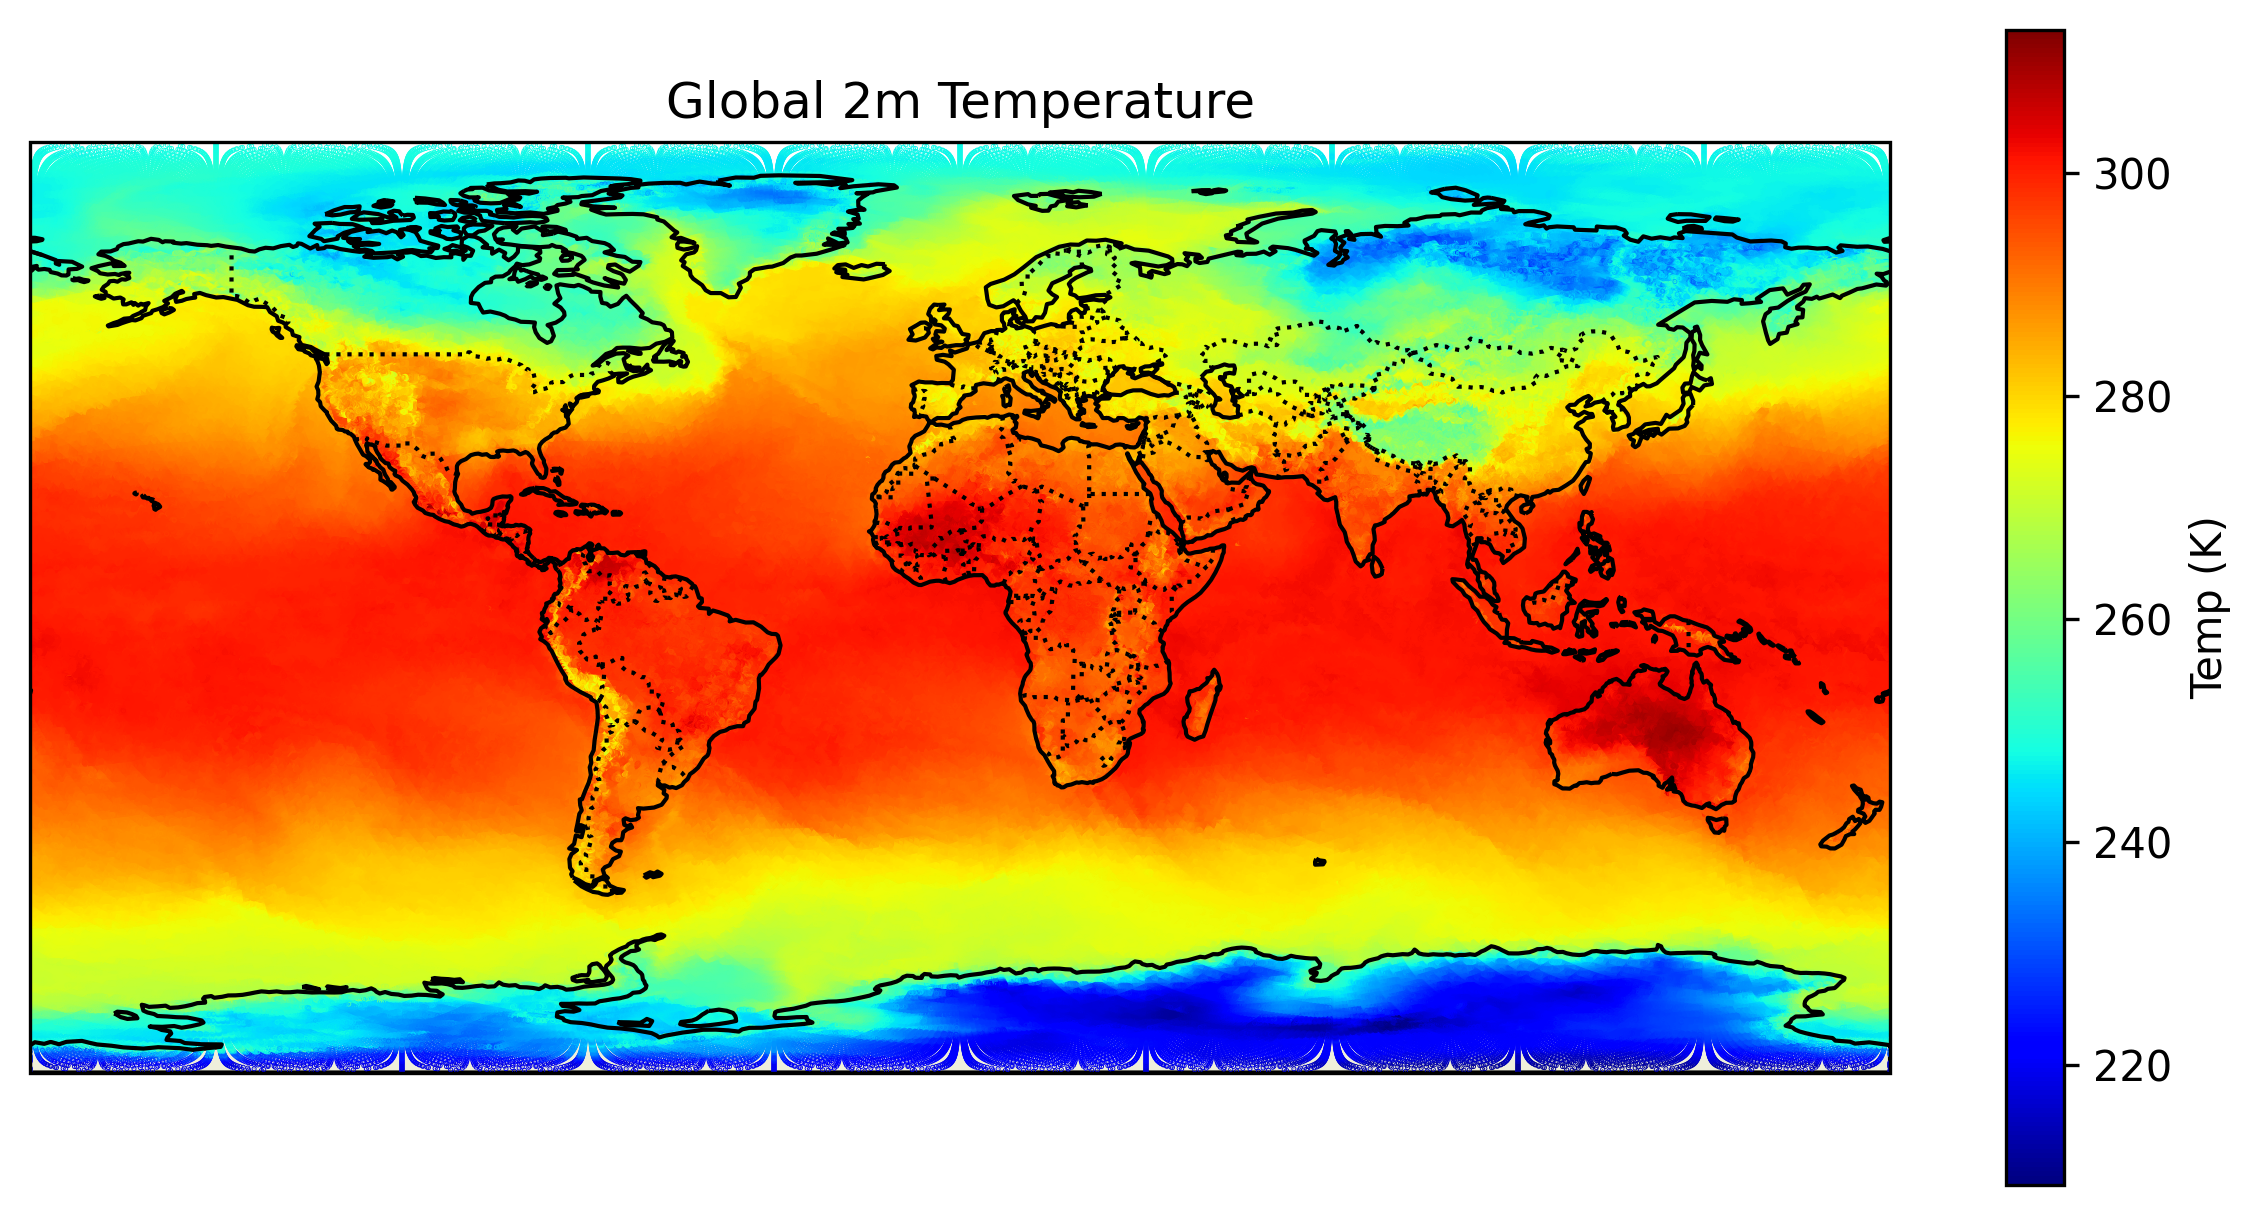
\includegraphics[width=\textwidth]{images/icon_t2m_global.png}
        \caption{Global 2m temperature field.}
        \label{fig:t2m_global_interp}
    \end{minipage}
    \hfill
    \begin{minipage}{0.4\textwidth}
        \centering
        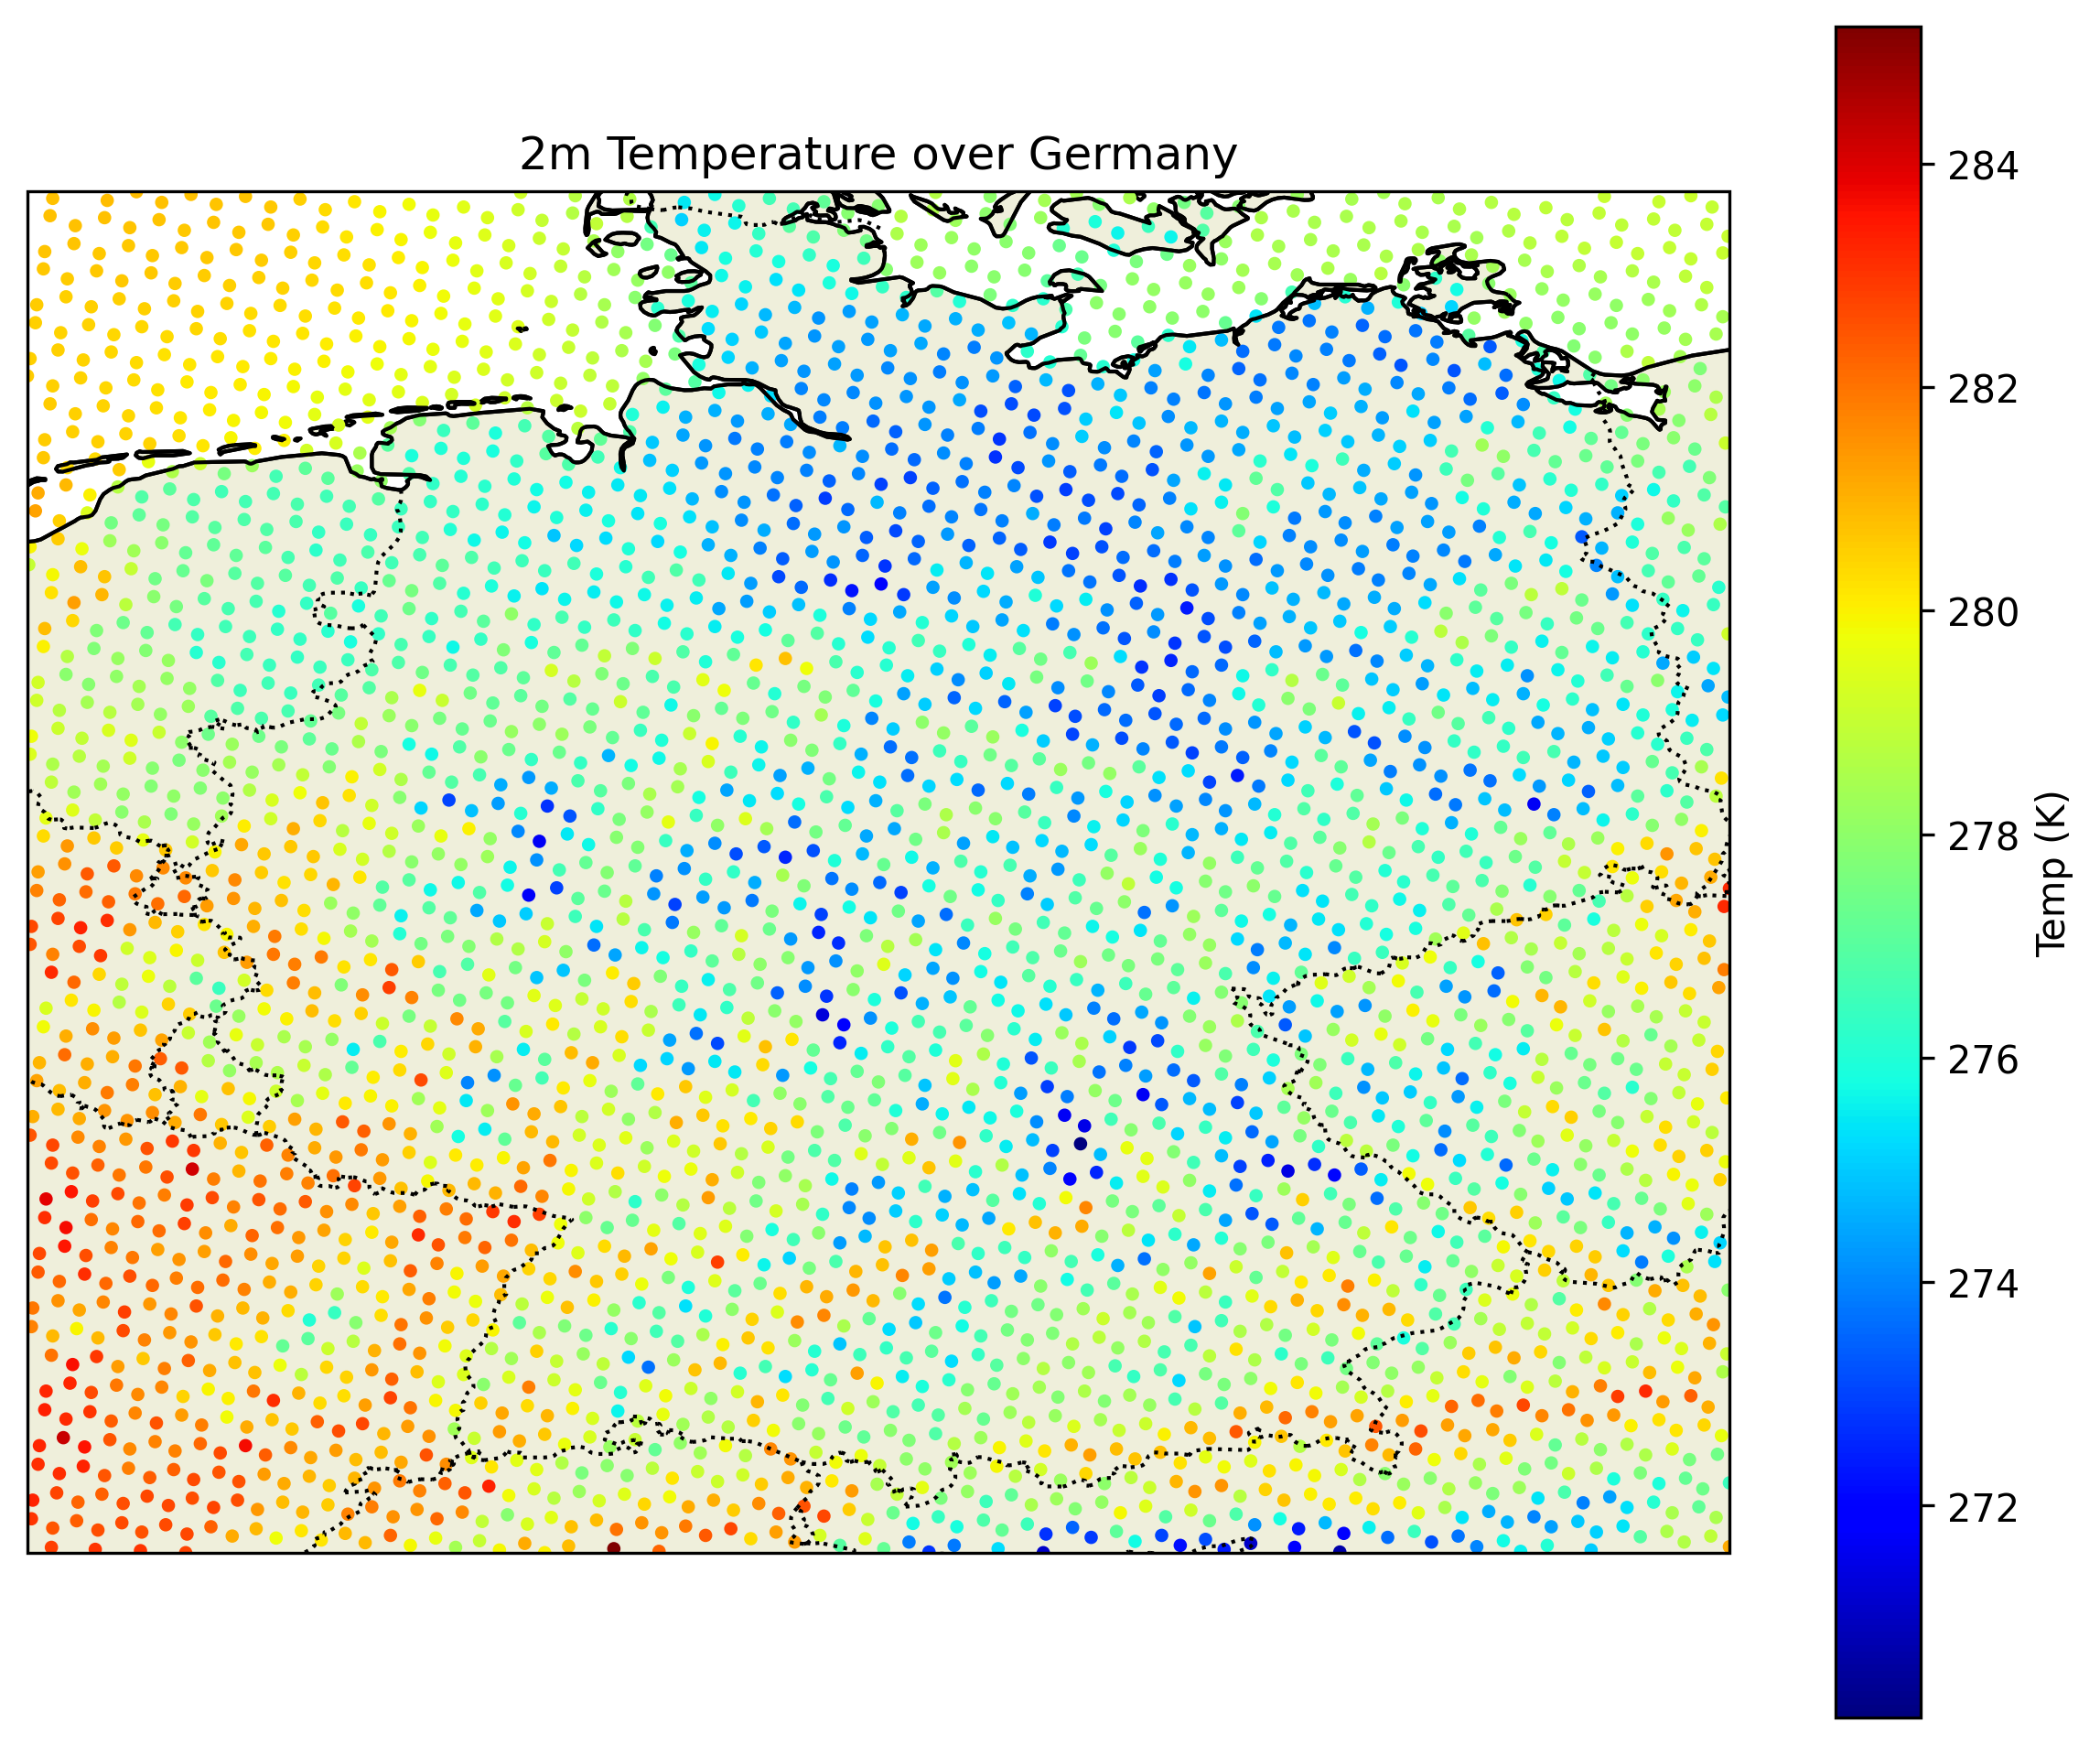
\includegraphics[width=\textwidth]{images/icon_t2m_germany.png}
        \caption{2m temperature field over Germany.}
        \label{fig:t2m_germany_interp}
    \end{minipage}
\end{figure}

\begin{figure}[ht]
    \centering
    \begin{minipage}{0.5\textwidth}
        \centering
        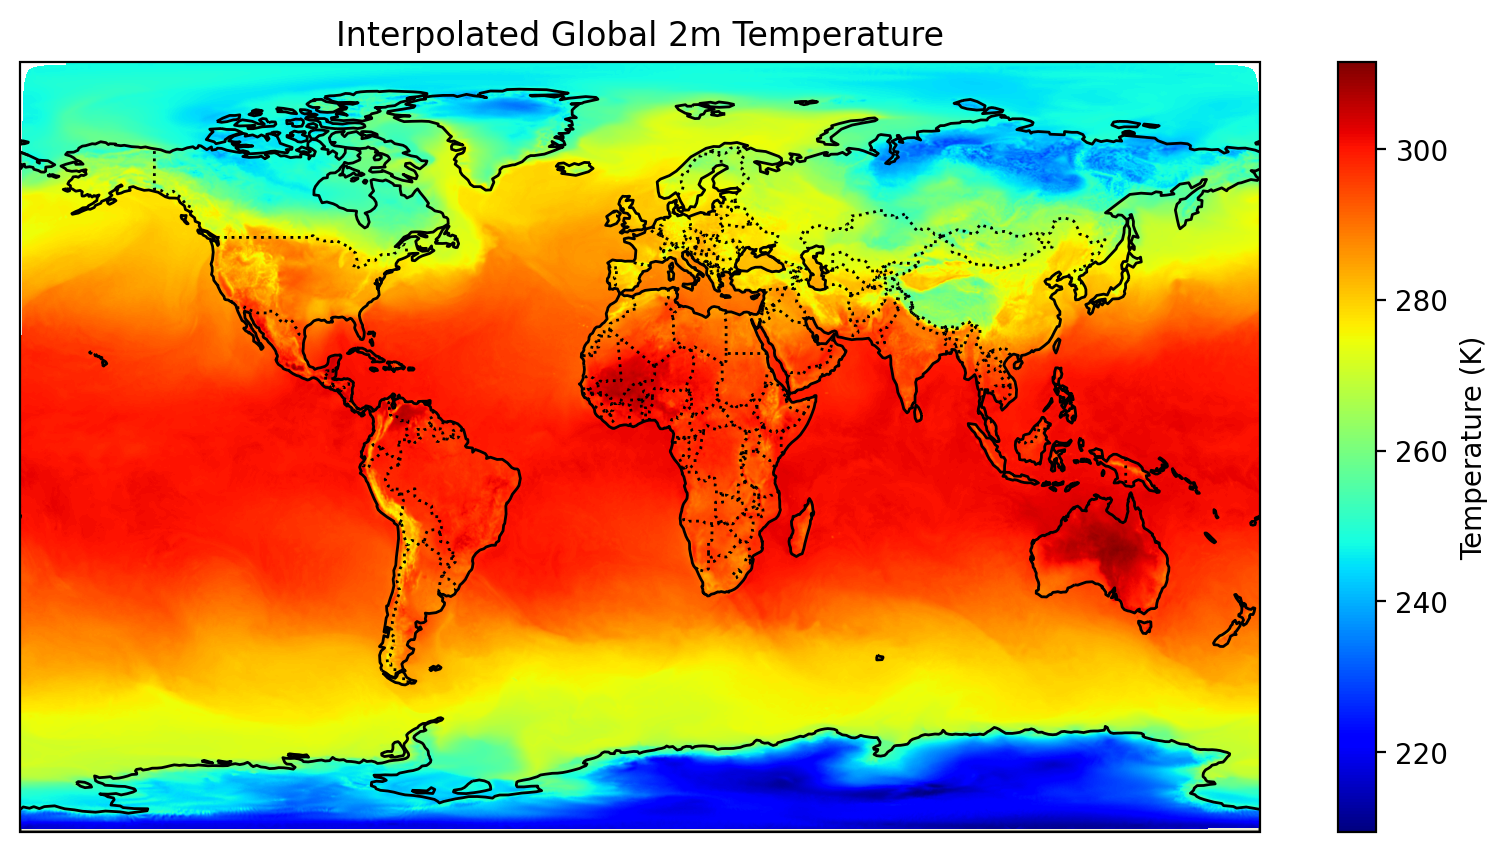
\includegraphics[width=\textwidth]{images/icon_t2m_global_interp.png}
        \caption{Interpolated global 2m temperature field.}
        \label{fig:t2m_global_interp}
    \end{minipage}
    \hfill
    \begin{minipage}{0.4\textwidth}
        \centering
        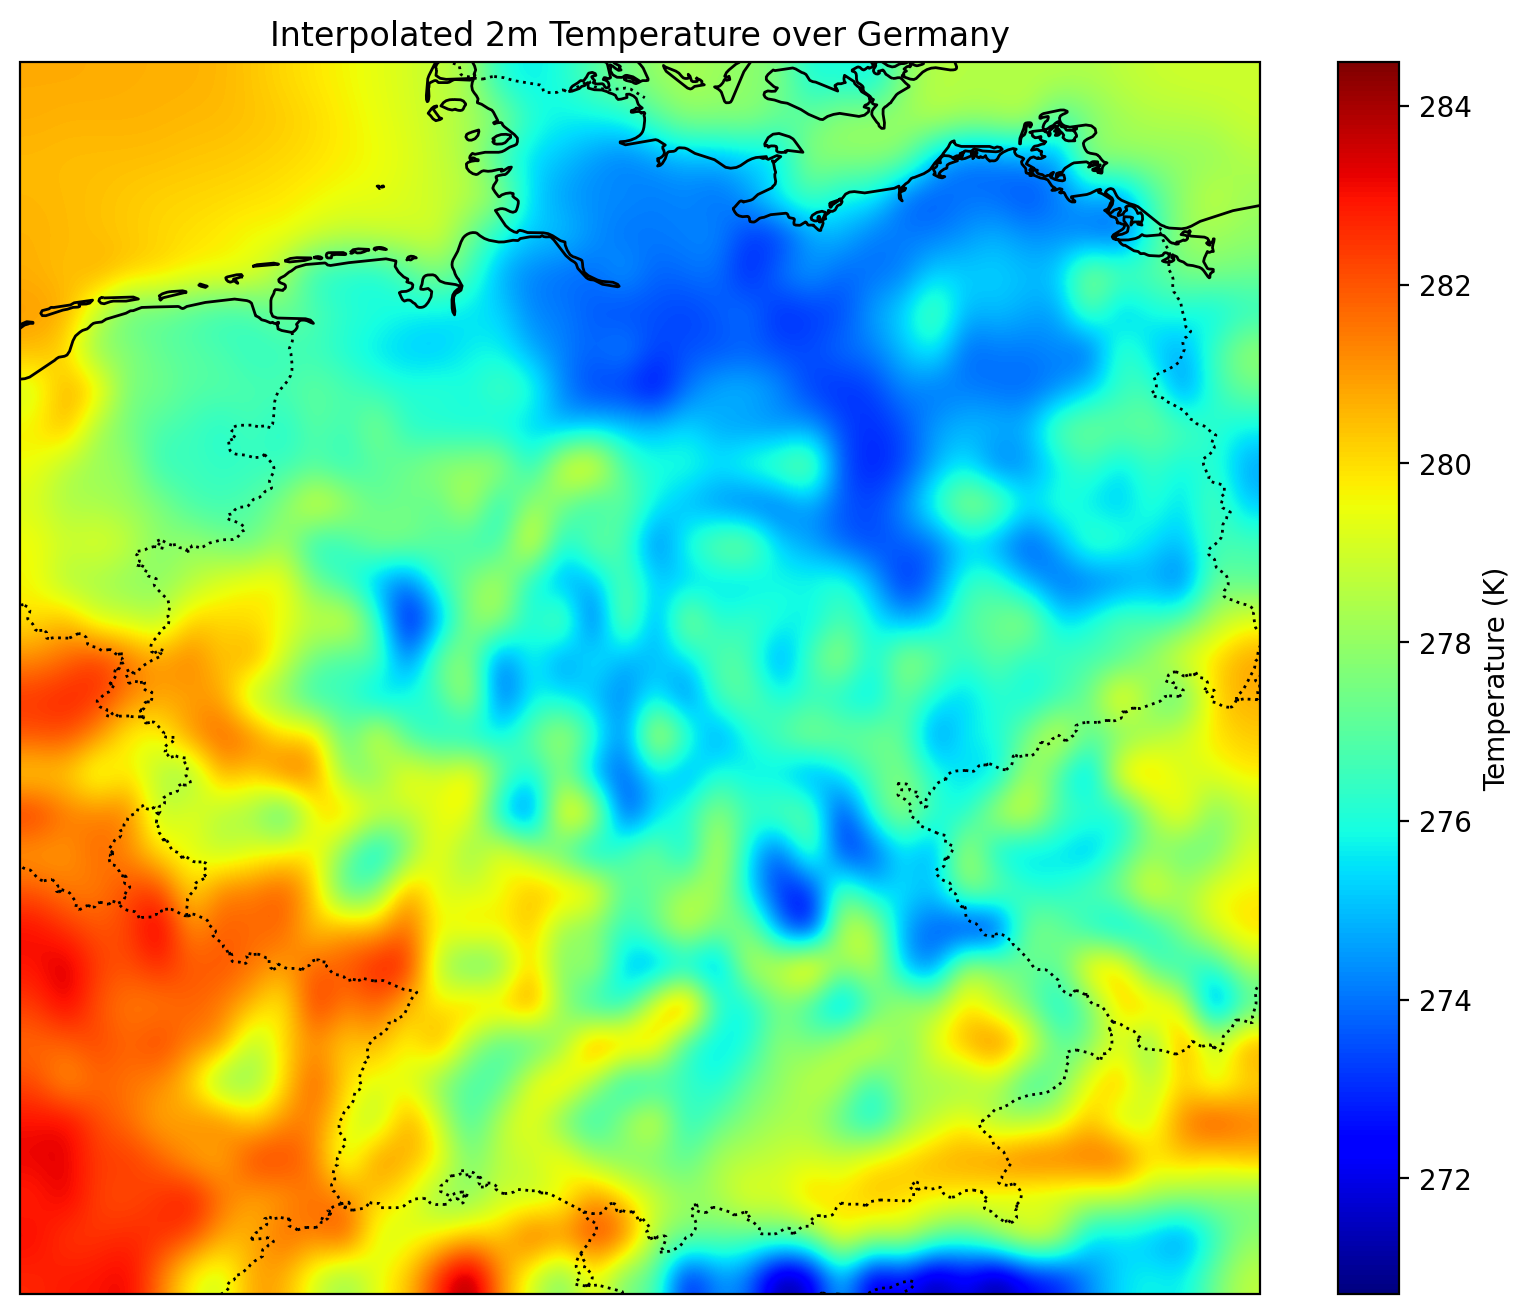
\includegraphics[width=\textwidth]{images/icon_t2m_germany_interp.png}
        \caption{Interpolated 2m temperature field over Germany.}
        \label{fig:t2m_germany_interp}
    \end{minipage}
\end{figure}

{\bf Interpolated Visualization of 2-Meter Temperature (T2M)}

To enhance the visualization of the 2-meter temperature field, we interpolate the scattered GRIB data onto a regular grid using cubic interpolation. This results in a smooth temperature field representation. The interpolation function is implemented as follows:

\begin{codeonly}{Interpolating T2M to a Regular Grid}
import numpy as np
from scipy.interpolate import griddata

def interpolate_to_grid(lat, lon, t2m, bbox, grid_res=0.25):
    """Interpolates T2M data onto a regular lat/lon grid."""
    latmin, latmax, lonmin, lonmax = bbox

    # Define a smooth regular grid
    grid_lat = np.arange(latmin, latmax, grid_res)
    grid_lon = np.arange(lonmin, lonmax, grid_res)
    lon_grid, lat_grid = np.meshgrid(grid_lon, grid_lat)

    # Use cubic interpolation for smooth output
    t2m_grid = griddata((lon, lat), t2m, (lon_grid, lat_grid), method='cubic')

    return lon_grid, lat_grid, t2m_grid
\end{codeonly}

Once the temperature field is interpolated, we visualize it using \texttt{matplotlib} and \texttt{cartopy}. The function for plotting the interpolated data is shown below:

\begin{codeonly}{Plotting Interpolated T2M}
import matplotlib.pyplot as plt
import cartopy.crs as ccrs
import cartopy.feature as cfeature

def plot_t2m_grid(lat, lon, t2m, bbox, title, fname):
    """Plots interpolated 2m temperature as a smooth heatmap."""
    lon_grid, lat_grid, t2m_grid = interpolate_to_grid(lat, lon, t2m, bbox)

    # Set reasonable aspect ratio based on bounding box size
    lon_range = bbox[3] - bbox[2]
    lat_range = bbox[1] - bbox[0]
    aspect_ratio = lon_range / lat_range
    figsize = (10, max(5, 10 / aspect_ratio))  # Maintain consistent width & prevent extreme height

    plt.figure(figsize=figsize)
    ax = plt.axes(projection=ccrs.PlateCarree())
    ax.set_extent([bbox[2], bbox[3], bbox[0], bbox[1]])
    ax.add_feature(cfeature.LAND, edgecolor='black')
    ax.add_feature(cfeature.COASTLINE)
    ax.add_feature(cfeature.BORDERS, linestyle=':')

    # Use smooth interpolation and correct aspect ratio
    img = ax.imshow(t2m_grid, extent=[bbox[2], bbox[3], bbox[0], bbox[1]], origin='lower',
                    cmap='jet', transform=ccrs.PlateCarree(), aspect='auto', interpolation='bicubic')

    plt.colorbar(img, label="Temperature (K)")
    plt.title(title)
    plt.savefig(fname, dpi=200, bbox_inches='tight')  # Reduce DPI for smaller file size
    plt.show()
\end{codeonly}

Using this interpolation approach, we generate the visualizations shown in Figures \ref{fig:t2m_global_interp} and \ref{fig:t2m_germany_interp} for the global and regional (Germany) temperature fields, see figure. 

\begin{recommendationbox}
Using libraries such as eccodes can be carried out in a very elementary way. At the same time, building packages is an important activity. Keep the balance, being able to do things elementary if necessary, while using packages to work efficiently. 
\end{recommendationbox}

%==============================================================================
%
%==============================================================================
\section{Accessing SYNOP Observation Files from NetCDF}

Observational weather data is often stored in the \emph{BUFR} (Binary Universal Form for the Representation of meteorological data) format, a widely used WMO standard. To facilitate data access, BUFR files are commonly converted into \emph{NetCDF} (Network Common Data Form), which provides a structured, self-describing format suitable for scientific applications.

NetCDF files containing SYNOP observations include essential meteorological variables such as temperature, pressure, humidity, wind speed, and cloud cover. Accessing these files requires a programming framework that can read NetCDF structures efficiently.

\begin{figure}[ht]
    \centering
    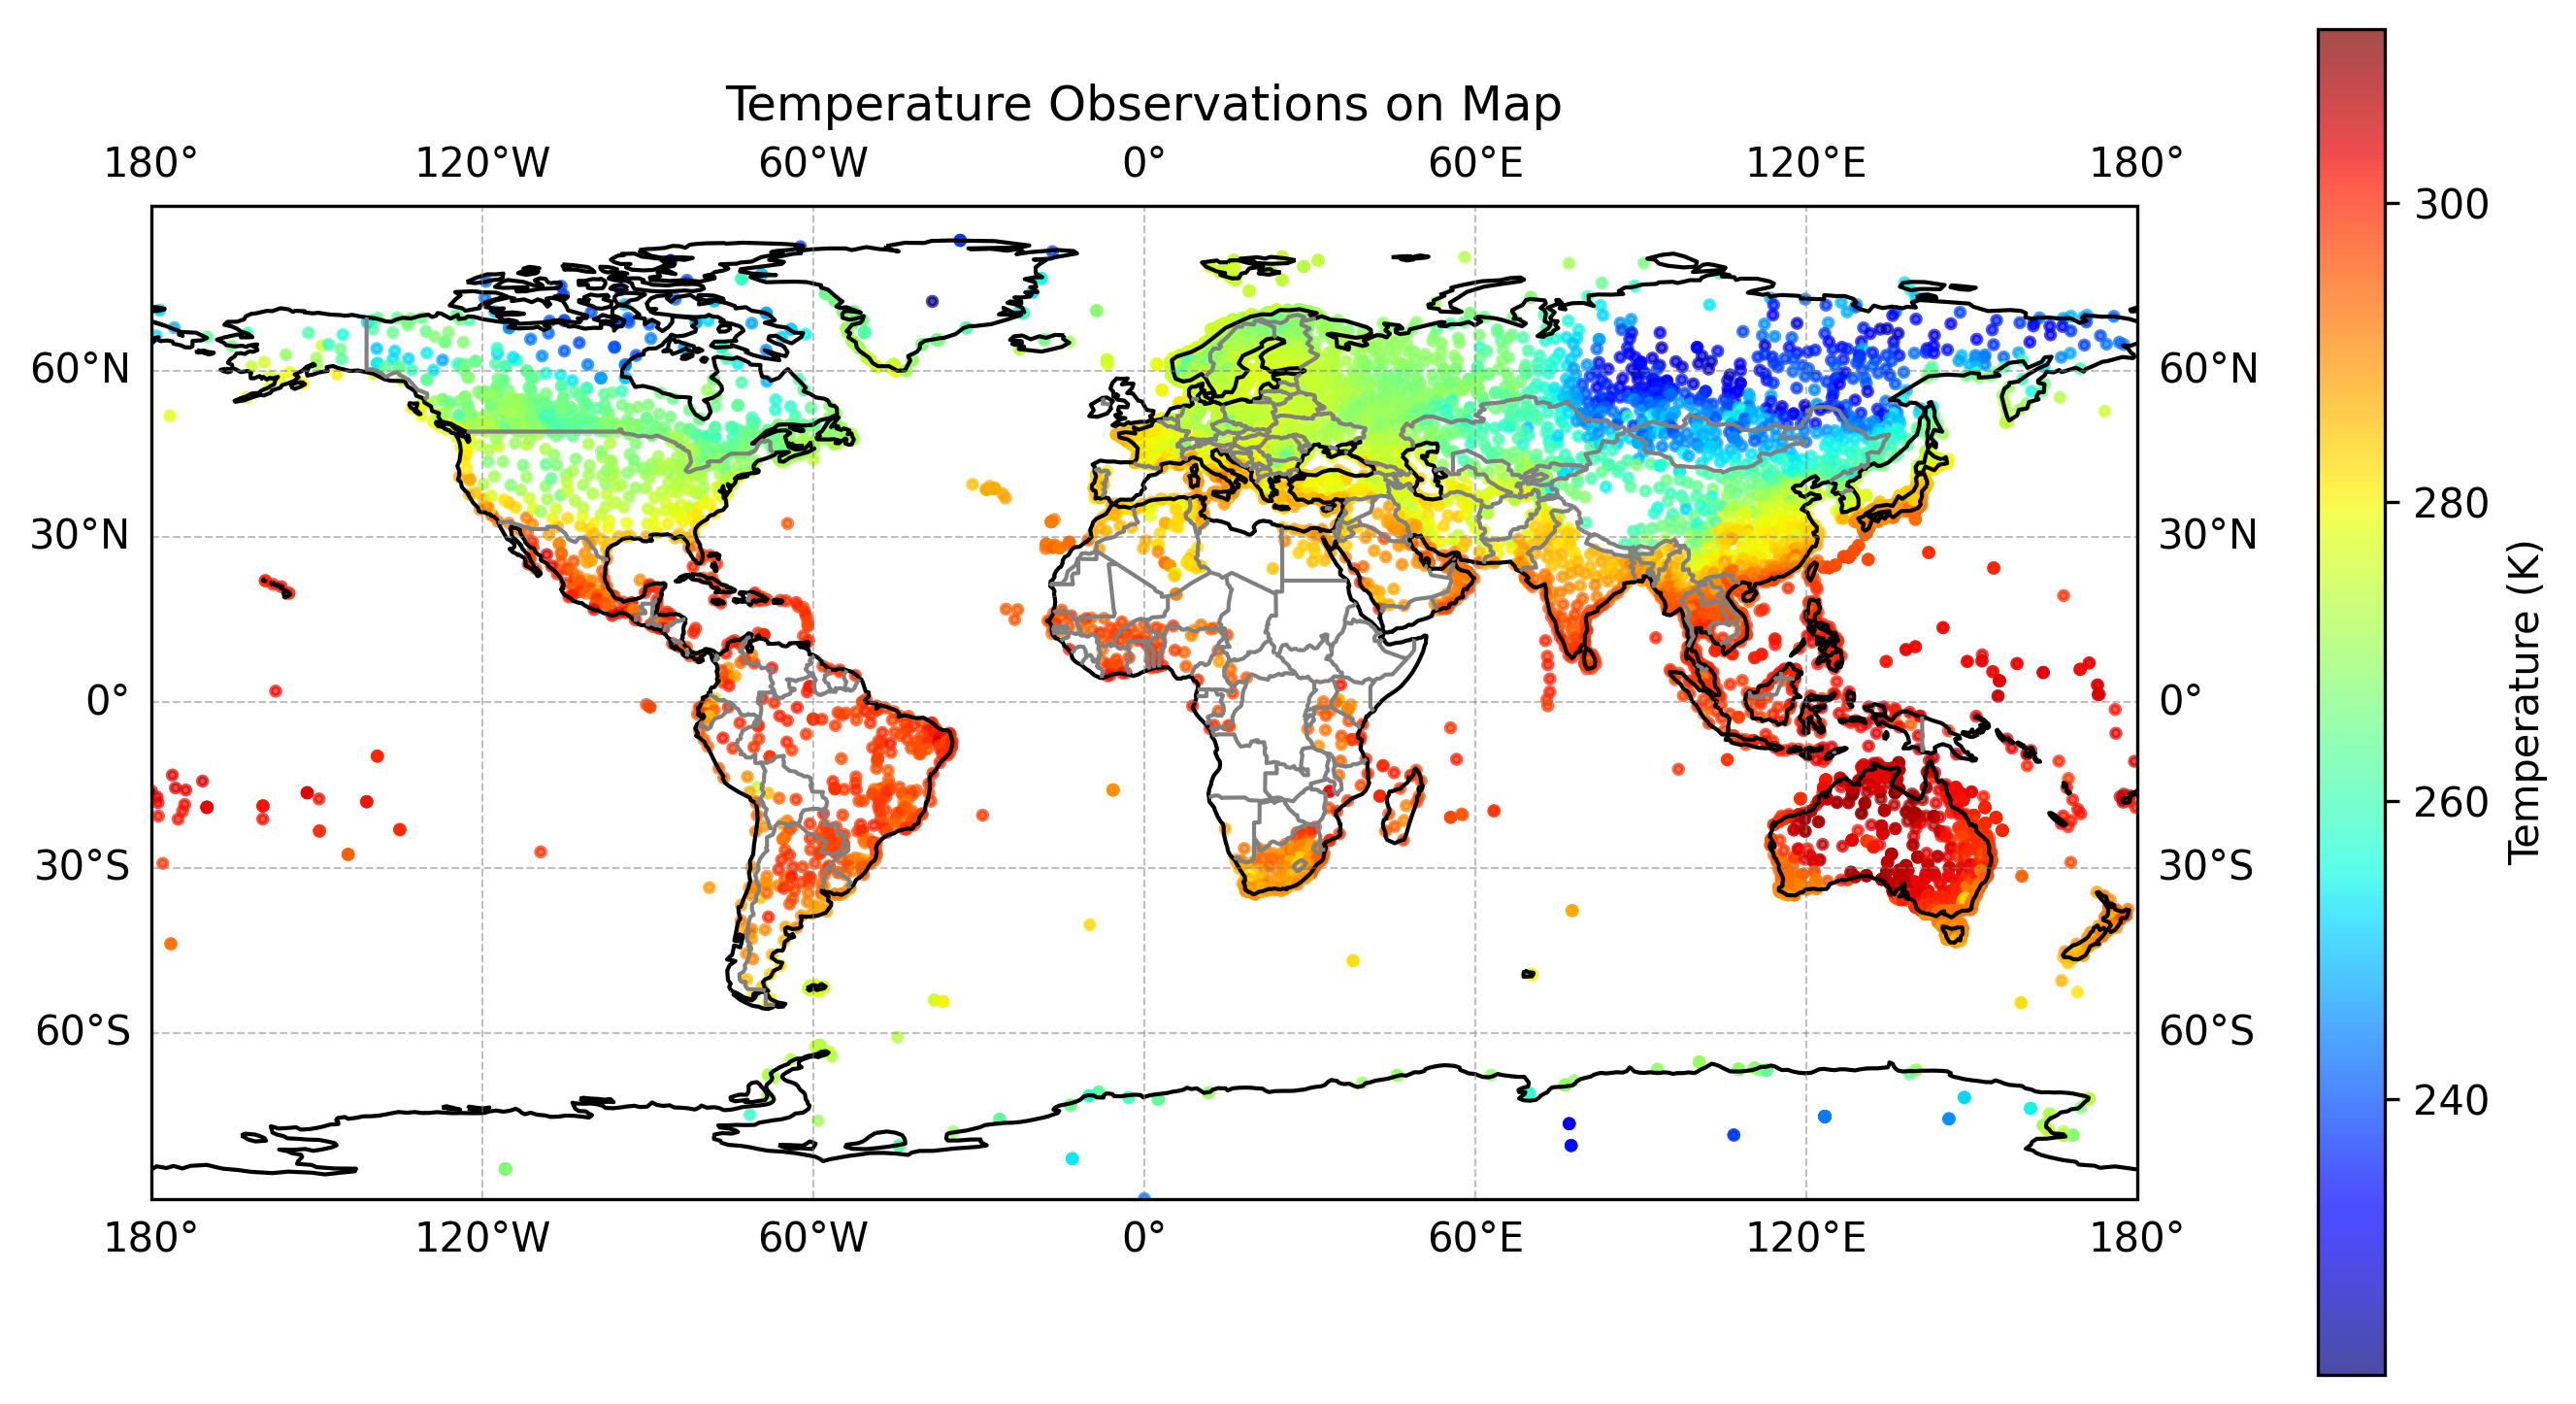
\includegraphics[width=0.9\textwidth]{images/synop.png}
    \caption{Scatter plot of SYNOP temperature observations}
    \label{fig:synop_plot}
\end{figure}

\textbf{Listing Variables in a NetCDF File}

To get an overview of the available variables, we use the following script:

\begin{codeonly}{Listing NetCDF Variables}
from netCDF4 import Dataset

def nc_list(file1):
    """
    Lists all variables in a given NetCDF file, displaying their names, dimensions, and descriptions.
    """
    ncfile = Dataset(file1, 'r')

    print("{:<4} {:40} {:>10} {:>10}  {:30}".format("No", "Varname", "shape1", "shape2", "Description"))
    print("-"*110)

    nc = 1
    for varname in ncfile.variables.keys():
        var = ncfile.variables[varname]
        description = var.long_name if hasattr(var, "long_name") else "N/A"
        dims = [len(ncfile.dimensions[dim]) for dim in var.dimensions]
        shape1 = dims[0] if len(dims) > 0 else ""
        shape2 = dims[1] if len(dims) > 1 else ""
        print("{:<4} {:40} {:>10} {:>10}  {:30}".format(nc, varname, shape1, shape2, description))  
        if nc % 10 == 0:
            print("-"*110)
        nc += 1
    ncfile.close()

file = "synop.nc"
nc_list(file)
\end{codeonly}

\textbf{Example Output}

\begin{codeonlysmall}{Example Output from nc\_list}
No   Varname                                      shape1     shape2  Description                   
--------------------------------------------------------------------------------------------------------------
1    edition_number                                11993             N/A                           
2    section1                                      11993         22  N/A                           
3    section2                                      11993         18  N/A                           
4    section1_master_table_nr                      11993             N/A                           
...
36   MLAH                                          11993             Latitude (high accuracy)      
37   MLOH                                          11993             Longitude (high accuracy)     
58   MTDBT                                         11993             Temperature/air temperature   
}
\end{codeonlysmall}

This function provides an overview of the variables, their dimensions, and descriptions if available, making it easier to understand the contents of the NetCDF file before further analysis.

\textbf{Frameworks for Accessing NetCDF Observations}

To work with SYNOP observations in NetCDF, we rely on established \emph{Python} libraries such as:
\begin{itemize}
    \item \texttt{netCDF4} -- Standard library for reading NetCDF data
    \item \texttt{numpy} -- Efficient numerical computations
    \item \texttt{matplotlib} -- Visualization of meteorological data
    \item \texttt{cartopy} -- Geospatial plotting on maps
\end{itemize}

\textbf{Reading SYNOP Data from NetCDF}

To extract observation data such as latitude, longitude, and temperature, we use the following Python script:

\begin{codeonly}{Reading latitude, longitude, and temperature from a NetCDF SYNOP file}
from netCDF4 import Dataset
import numpy as np

def read_synop_data(filename):
    """Reads latitude (MLAH), longitude (MLOH), and temperature (MTDBT) from a NetCDF file."""
    ncfile = Dataset(filename, 'r')
    
    lats = ncfile.variables["MLAH"][:]
    lons = ncfile.variables["MLOH"][:]
    temps = ncfile.variables["MTDBT"][:]
    
    ncfile.close()
    return np.array(lats), np.array(lons), np.array(temps)

# Example usage
lats, lons, temps = read_synop_data("synop.nc")
print("Latitudes:", lats[:5])
print("Longitudes:", lons[:5])
print("Temperatures:", temps[:5])
\end{codeonly}

\textbf{Filtering Missing Values}

NetCDF files contain default missing values, e.g., $9.96921\times10^{36}$. Before using the data, these values should be filtered out, here we employ a simple threshold:

\begin{codeonly}{Filtering large missing values in SYNOP NetCDF data}
def filter_missing_values(temps, threshold=1e+20):
    """Removes large default missing values from temperature data."""
    return temps[temps < threshold]

# Example usage
temps_filtered = filter_missing_values(temps)
\end{codeonly}

\textbf{Visualizing Observations on a Map}

For an intuitive representation of SYNOP data, we can plot temperature observations on a map:

\begin{codeonly}{Scatter plot of SYNOP temperature observations}
import numpy as np
import matplotlib.pyplot as plt
import cartopy.crs as ccrs
import cartopy.feature as cfeature

def plot_temperature_map(lats, lons, temps, filename="synop.png", threshold=1e+20):
    """Plots temperature observations on a map, removes large missing values, ensures proper colorbar spacing, and saves the figure."""

    # Filter out large missing values
    valid_mask = (temps < threshold) & np.isfinite(temps)
    lats, lons, temps = lats[valid_mask], lons[valid_mask], temps[valid_mask]

    # Create figure with proper aspect ratio
    fig, ax = plt.subplots(figsize=(10, 6), subplot_kw={'projection': ccrs.PlateCarree()})

    # Scatter plot with properly scaled colorbar
    scatter = ax.scatter(lons, lats, c=temps, cmap='coolwarm', s=5, alpha=0.7, transform=ccrs.PlateCarree())

    # Add map features
    ax.coastlines()
    ax.add_feature(cfeature.BORDERS, edgecolor='gray')
    ax.gridlines(draw_labels=True, linewidth=0.5, color='gray', alpha=0.5, linestyle='--')

    # Add colorbar with better spacing
    cbar = plt.colorbar(scatter, ax=ax, fraction=0.04, pad=0.08)
    cbar.set_label("Temperature (K)")

    # Set title
    plt.title("Temperature Observations on Map")

    # Save and show the plot
    plt.savefig(filename, dpi=300, bbox_inches="tight")
    plt.show()

# Example usage
plot_temperature_map(lats, lons, temps)
\end{codeonly}

This script generates a scatter plot where each SYNOP observation is plotted on a geographical map, see Figure \ref{fig:synop_plot}. The color of each point represents the observed temperature, providing a clear spatial overview of meteorological conditions.


%==============================================================================
%
%==============================================================================
\section{Analysing AIREP Feedback Files in NetCDF Format}

Aircraft Reports (AIREP) provide vital meteorological observations from airborne sources. These reports contain real-time measurements of parameters such as temperature, wind speed, pressure, and humidity. The data is often stored in \emph{BUFR} (Binary Universal Form for the Representation of meteorological data) format and later converted into \emph{NetCDF} (Network Common Data Form) for easier access and processing.

\textbf{Structure of AIREP NetCDF Files}

AIREP feedback files in NetCDF format consist of multiple dimensions and variables. The primary dimensions include:

\begin{itemize}
    \item \texttt{d\_hdr} -- Number of header entries (stations, timestamps, metadata)
    \item \texttt{d\_body} -- Number of observed variables (measurements at different levels)
    \item \texttt{d\_veri} -- Number of verification entries
\end{itemize}

Each observation is associated with key metadata, including:

\begin{itemize}
    \item \texttt{lat}, \texttt{lon} -- Geographic coordinates of the observation
    \item \texttt{varno} -- Variable number defining the type of measurement
    \item \texttt{obs} -- Observed value, bias-corrected
    \item \texttt{plevel} -- Pressure level at which the observation was made
    \item \texttt{veri\_data} -- Corresponding modeled values for verification
\end{itemize}

\textbf{Inspecting Variables in AIREP NetCDF Files}

To get an overview of the available variables, the following Python function lists all variables along with their dimensions and descriptions:

\begin{codeonly}{Listing NetCDF Variables in AIREP Files}
from netCDF4 import Dataset

def nc_list(file1):
    """
    Lists all variables in a given NetCDF file, displaying their names, dimensions, and descriptions.
    
    Parameters:
    file1 (str): Path to the NetCDF file.

    Output:
    Prints a formatted table of variables with their dimensions and descriptions.
    """
    ncfile = Dataset(file1, 'r')

    print("{:<4} {:40} {:>10} {:>10}  {:30}".format("No", "Varname", "shape1", "shape2", "Description")) 
    print("-" * 110)

    nc = 1
    for varname in ncfile.variables.keys():
        var = ncfile.variables[varname]
        
        # Retrieve description from correct attribute
        description = getattr(var, "longname", "N/A")

        # Get variable dimensions
        dims = [len(ncfile.dimensions[dim]) for dim in var.dimensions]

        # Ensure at least 2 shape values
        shape1 = dims[0] if len(dims) > 0 else ""
        shape2 = dims[1] if len(dims) > 1 else ""

        print("{:<4} {:40} {:>10} {:>10}  {:30}".format(nc, varname, shape1, shape2, description))

        if nc % 10 == 0: 
            print("-" * 110)
        nc += 1

    ncfile.close()

# Example usage
file = "monAIREP.nc"
nc_list(file)
\end{codeonly}

\begin{codeonlysmall}{Example Output of nc\_list}
No   Varname                       shape1     shape2  Description                   
----------------------------------------------------------------------------------------------------
1    i_body                         37198             index of 1st entry in report body
2    l_body                         37198             number of entries in report body
3    n_level                        37198             number of levels in report    
4    data_category                  37198             BUFR4 data category           
5    sub_category                   37198             BUFR4 data sub-category       
6    center                         37198             station processing center     
7    sub_center                     37198             station processing sub-center 
8    obstype                        37198             observation type              
9    codetype                       37198             code type                     
10   ident                          37198             station or satellite id as integer
----------------------------------------------------------------------------------------------------
11   statid                         37198         10  station id as character string
12   lat                            37198             latitude                      
13   lon                            37198             longitude                     
14   time                           37198             observation minus reference time
15   time_nomi                      37198             nominal (synoptic) minus reference time
16   time_dbase                     37198             data base minus reference time
17   z_station                      37198             station height                
18   z_modsurf                      37198             model surface height          
19   r_state                        37198             status of the report          
20   r_flags                        37198             report quality check flags    
----------------------------------------------------------------------------------------------------
21   r_check                        37198             check which raised the report status flag value
22   sta_corr                       37198             station correction indicator  
23   index_x                        37198             index x of model grid point assigned to report
24   index_y                        37198             index y of model grid point assigned to report
25   mdlsfc                         37198             model surface characteristics 
26   instype                        37198             station type or satellite instrument type
27   sun_zenit                      37198             sun zenith angle              
28   phase                          37198             aircraft phase                
29   tracking                       37198             tracking technique            
30   obs_id                         37198             unique observation id         
----------------------------------------------------------------------------------------------------
31   source                         37198             input file number             
32   record                         37198             record number in the input file
33   subset                         37198             subset number in the record   
34   dbkz                           37198             DWD data base id              
35   index_d                        37198             model grid diamond index assigned to report
36   varno                         187770             type of the observed quantity 
37   obs                           187770             bias corrected observation    
38   bcor                          187770             bias correction, corrected minus observed
39   level                         187770             level of observation          
40   level_typ                     187770             type of level information     
----------------------------------------------------------------------------------------------------
41   level_sig                     187770             level significance            
42   state                         187770             status of the observation     
43   flags                         187770             observation quality check flags
44   check                         187770             check which raised the observation status flag value
45   e_o                           187770             observational error           
46   qual                          187770             observation confidence from data provider
47   plevel                        187770             nominal pressure level        
48   veri_data                          5     187770  modelled quantity (as indicated by veri_ens_member)
49   veri_model                         5         10  model used for verification, e.g. COSMO, GME ...
50   veri_run_type                      5             type of model run             
----------------------------------------------------------------------------------------------------
51   veri_run_class                     5             class of model run            
...
\end{codeonlysmall}

\textbf{Extracting AIREP Observations from NetCDF}

To retrieve latitude, longitude, and observation values, we use the following function:

\begin{codeonly}{Reading AIREP Observations from NetCDF}
from netCDF4 import Dataset
import numpy as np
import matplotlib.pyplot as plt
import cartopy.crs as ccrs
import cartopy.feature as cfeature

def read_airep_data(filename, varno, extra_vars=None):
    """Reads latitude, longitude, selected observations, and additional variables from a NetCDF file."""
    if extra_vars is None:
        extra_vars = []

    ncfile = Dataset(filename, 'r')
    
    # Read header-level variables
    lat = ncfile.variables["lat"][:]
    lon = ncfile.variables["lon"][:]
    
    # Read body-level variables
    varno_all = ncfile.variables["varno"][:]
    obs_all = ncfile.variables["obs"][:]
    l_body = ncfile.variables["l_body"][:]

    # Expand lat/lon to match body-level observations
    ni = len(l_body)
    ie = np.repeat(range(0, ni), l_body)
    
    # Find matching variable numbers
    idx = np.where(varno_all == varno)[0]
    
    # Filter lat, lon, obs
    lat_filtered = lat[ie[idx]]
    lon_filtered = lon[ie[idx]]
    obs_filtered = obs_all[idx]

    # Read extra variables if requested
    extra_data = {}
    for var in extra_vars:
        if var in ncfile.variables:
            var_data = ncfile.variables[var][:]
            extra_data[var] = var_data[idx] if var_data.shape[0] == len(varno_all) else var_data[ie[idx]]
        else:
            print(f"Warning: Variable '{var}' not found in NetCDF file.")

    ncfile.close()
    return lat_filtered, lon_filtered, obs_filtered, extra_data

\end{codeonly}

\begin{figure}[ht]
    \centering
    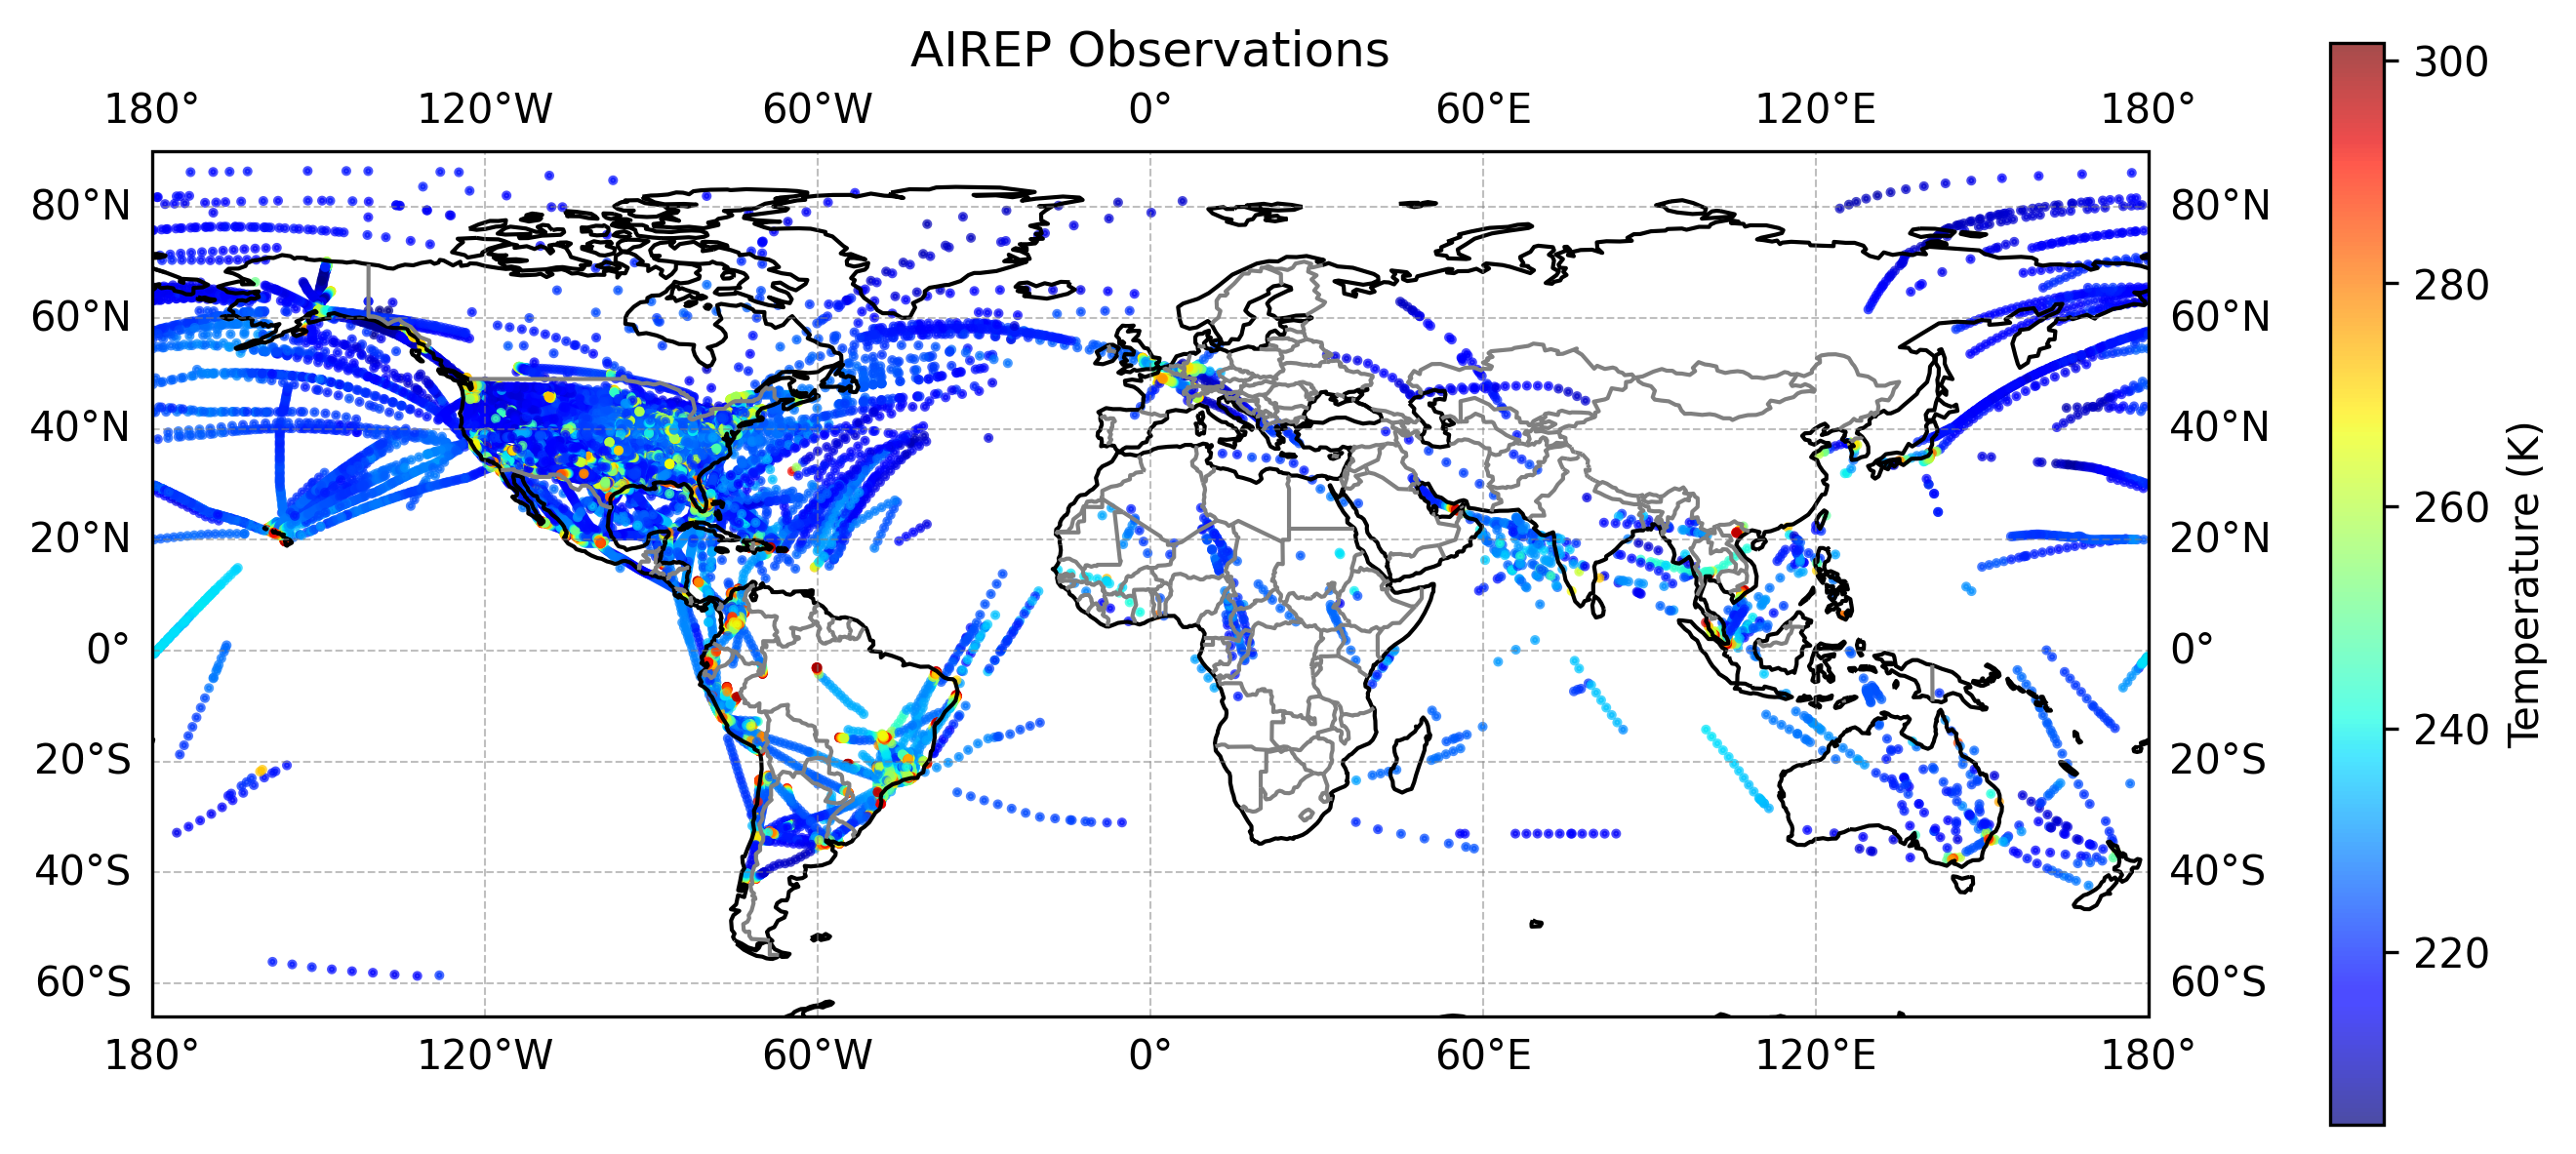
\includegraphics[width=0.9\textwidth]{images/airep.png}
    \caption{Scatter plot of AIREP observations}
    \label{fig:airep_plot}
\end{figure}

\textbf{Filtering Out Missing Values and Outliers}

AIREP NetCDF files may contain default missing values (e.g., $9.96921\times10^{36}$) and unrealistic outliers. We filter them as follows:

\begin{codeonly}{Filtering Missing Values and Outliers in AIREP Data}
def filter_airep_data(lats, lons, obs, threshold=1e+20):
    """Filters AIREP observations by removing missing values and out-of-range temperatures."""
    valid_mask = (obs < threshold) & np.isfinite(obs)
    lats, lons, obs = lats[valid_mask], lons[valid_mask], obs[valid_mask]
    temp_min, temp_max = 180, 320
    physical_mask = (obs >= temp_min) & (obs <= temp_max)
    return lats[physical_mask], lons[physical_mask], obs[physical_mask]
\end{codeonly}

\textbf{Visualizing AIREP Observations on a Map}

For a better understanding of the spatial distribution of AIREP observations, we plot them on a map using the following function:

\begin{codeonly}{Plotting AIREP Observations on a Map}
def plot_airep_map(lats, lons, obs, filename="airep.png"):
    """Plots AIREP observations on a map after filtering out-of-range temperatures."""

    fig, ax = plt.subplots(figsize=(10, 6), subplot_kw={'projection': ccrs.PlateCarree()})

    scatter = ax.scatter(lons, lats, c=obs, cmap='jet', s=2, alpha=0.7, transform=ccrs.PlateCarree())

    ax.coastlines()
    ax.add_feature(cfeature.BORDERS, edgecolor='gray')
    ax.gridlines(draw_labels=True, linewidth=0.5, color='gray', alpha=0.5, linestyle='--')

    # Ensure the colorbar does not exceed figure height
    cbar = fig.colorbar(scatter, ax=ax, orientation='vertical', fraction=0.04, pad=0.08, shrink=0.8)
    cbar.set_label("Temperature (K)")

    plt.title("AIREP Observations")
    plt.savefig(filename, dpi=300, bbox_inches="tight")
    plt.show()

# Example usage
lats_filtered, lons_filtered, obs_filtered = filter_airep_data(lats, lons, obs)
plot_airep_map(lats_filtered, lons_filtered, obs_filtered)
\end{codeonly}


The visualization of Figure \ref{fig:airep_plot} allows for a quick assessment of the coverage and accuracy of aircraft-derived meteorological data.

\begin{figure}[ht]
    \centering
    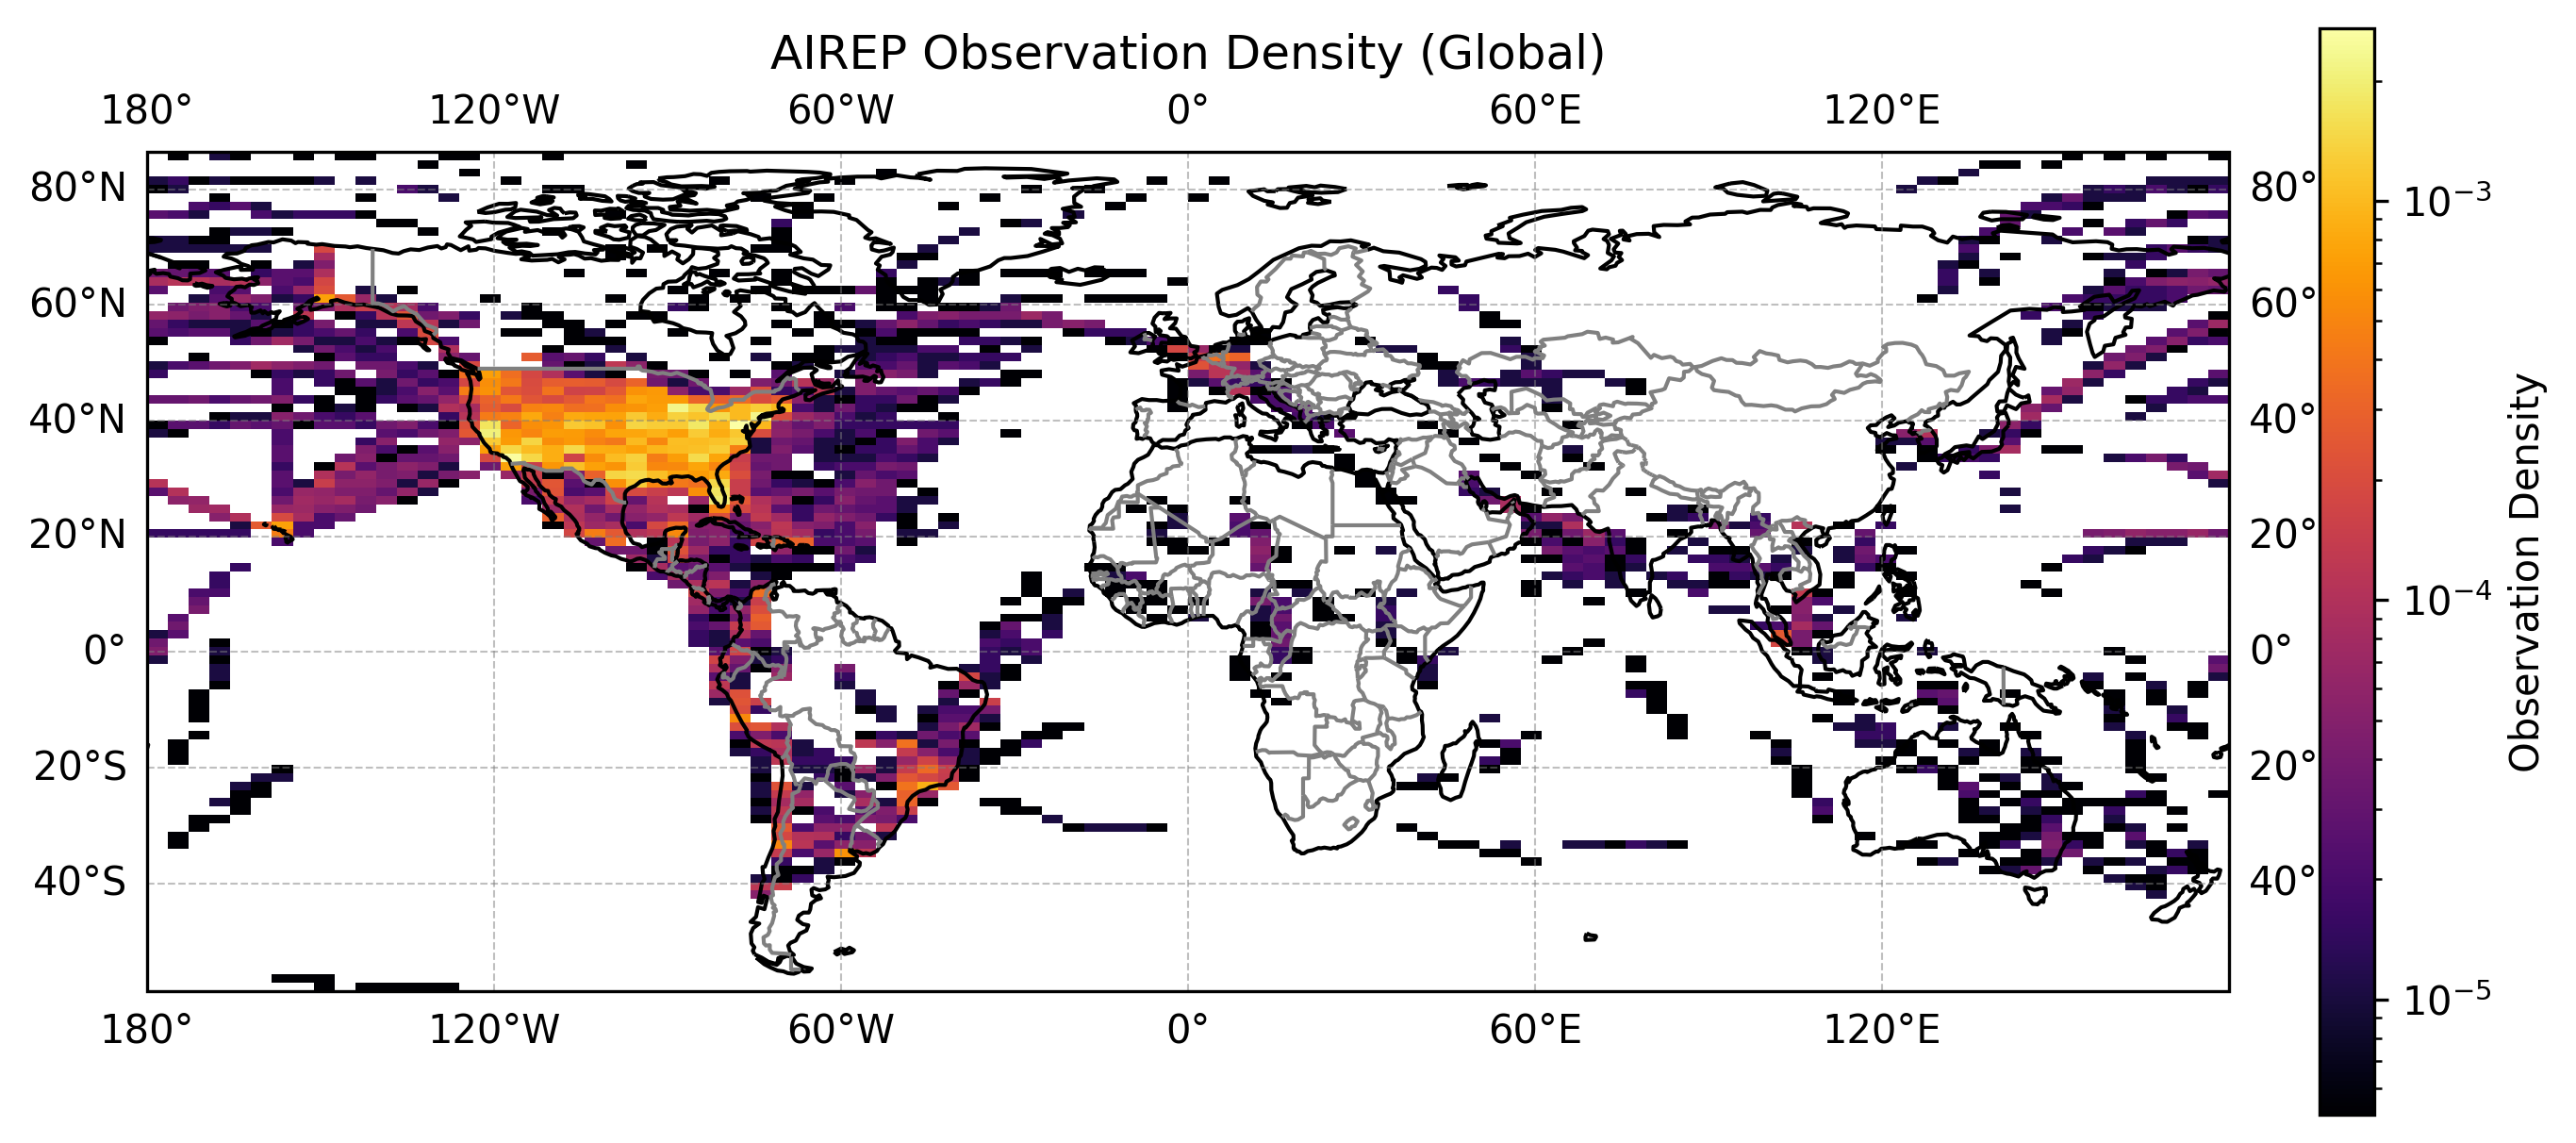
\includegraphics[width=0.9\textwidth]{images/airep_global_density.png}
    \caption{AIREP density in its horizontal distribution, while daytime in the US.}
    \label{fig:airep_plot}
\end{figure}


We can now analyse these data, for example by visualization of measurement density in horizontal or vertical distribution. 

\begin{codeonly}{Global AIREP Density Visualization}
import matplotlib.pyplot as plt
import cartopy.crs as ccrs
import cartopy.feature as cfeature
import numpy as np
from scipy.stats import gaussian_kde
from netCDF4 import Dataset

def plot_global_density(lats, lons,
                        filename="airep_global_density.png"):
    """Generates a density plot of AIREP observations on a world map 
    with an optimized colormap."""
    fig, ax = plt.subplots(figsize=(10, 6),
                           subplot_kw={'projection': ccrs.PlateCarree()})
    
    # Compute 2D histogram
    hist, xedges, yedges = np.histogram2d(lons, lats,
                                          bins=100, density=True)
    
    # Use a perceptually uniform colormap (e.g., 'inferno')
    pcm = ax.pcolormesh(xedges, yedges, hist.T, cmap='inferno',
                        norm=plt.matplotlib.colors.LogNorm(
                            vmin=hist[hist > 0].min(),
                            vmax=hist.max()),
                        transform=ccrs.PlateCarree())
    
    ax.coastlines()
    ax.add_feature(cfeature.BORDERS, edgecolor='gray')
    ax.gridlines(draw_labels=True, linewidth=0.5,
                 color='gray', alpha=0.5, linestyle='--')
    
    # Adjust padding to ensure axis does not crowd the figure
    plt.subplots_adjust(left=0.1, right=0.9, top=0.9, bottom=0.1)
    
    # Ensure colorbar does not exceed figure size
    cbar = fig.colorbar(pcm, ax=ax, orientation='vertical',
                        fraction=0.04, pad=0.04, shrink=0.8)
    cbar.set_label("Observation Density")
    
    plt.title("AIREP Observation Density (Global)")
    plt.savefig(filename, dpi=300, bbox_inches="tight")
    plt.show()
\end{codeonly}


\begin{figure}[ht]
    \centering
    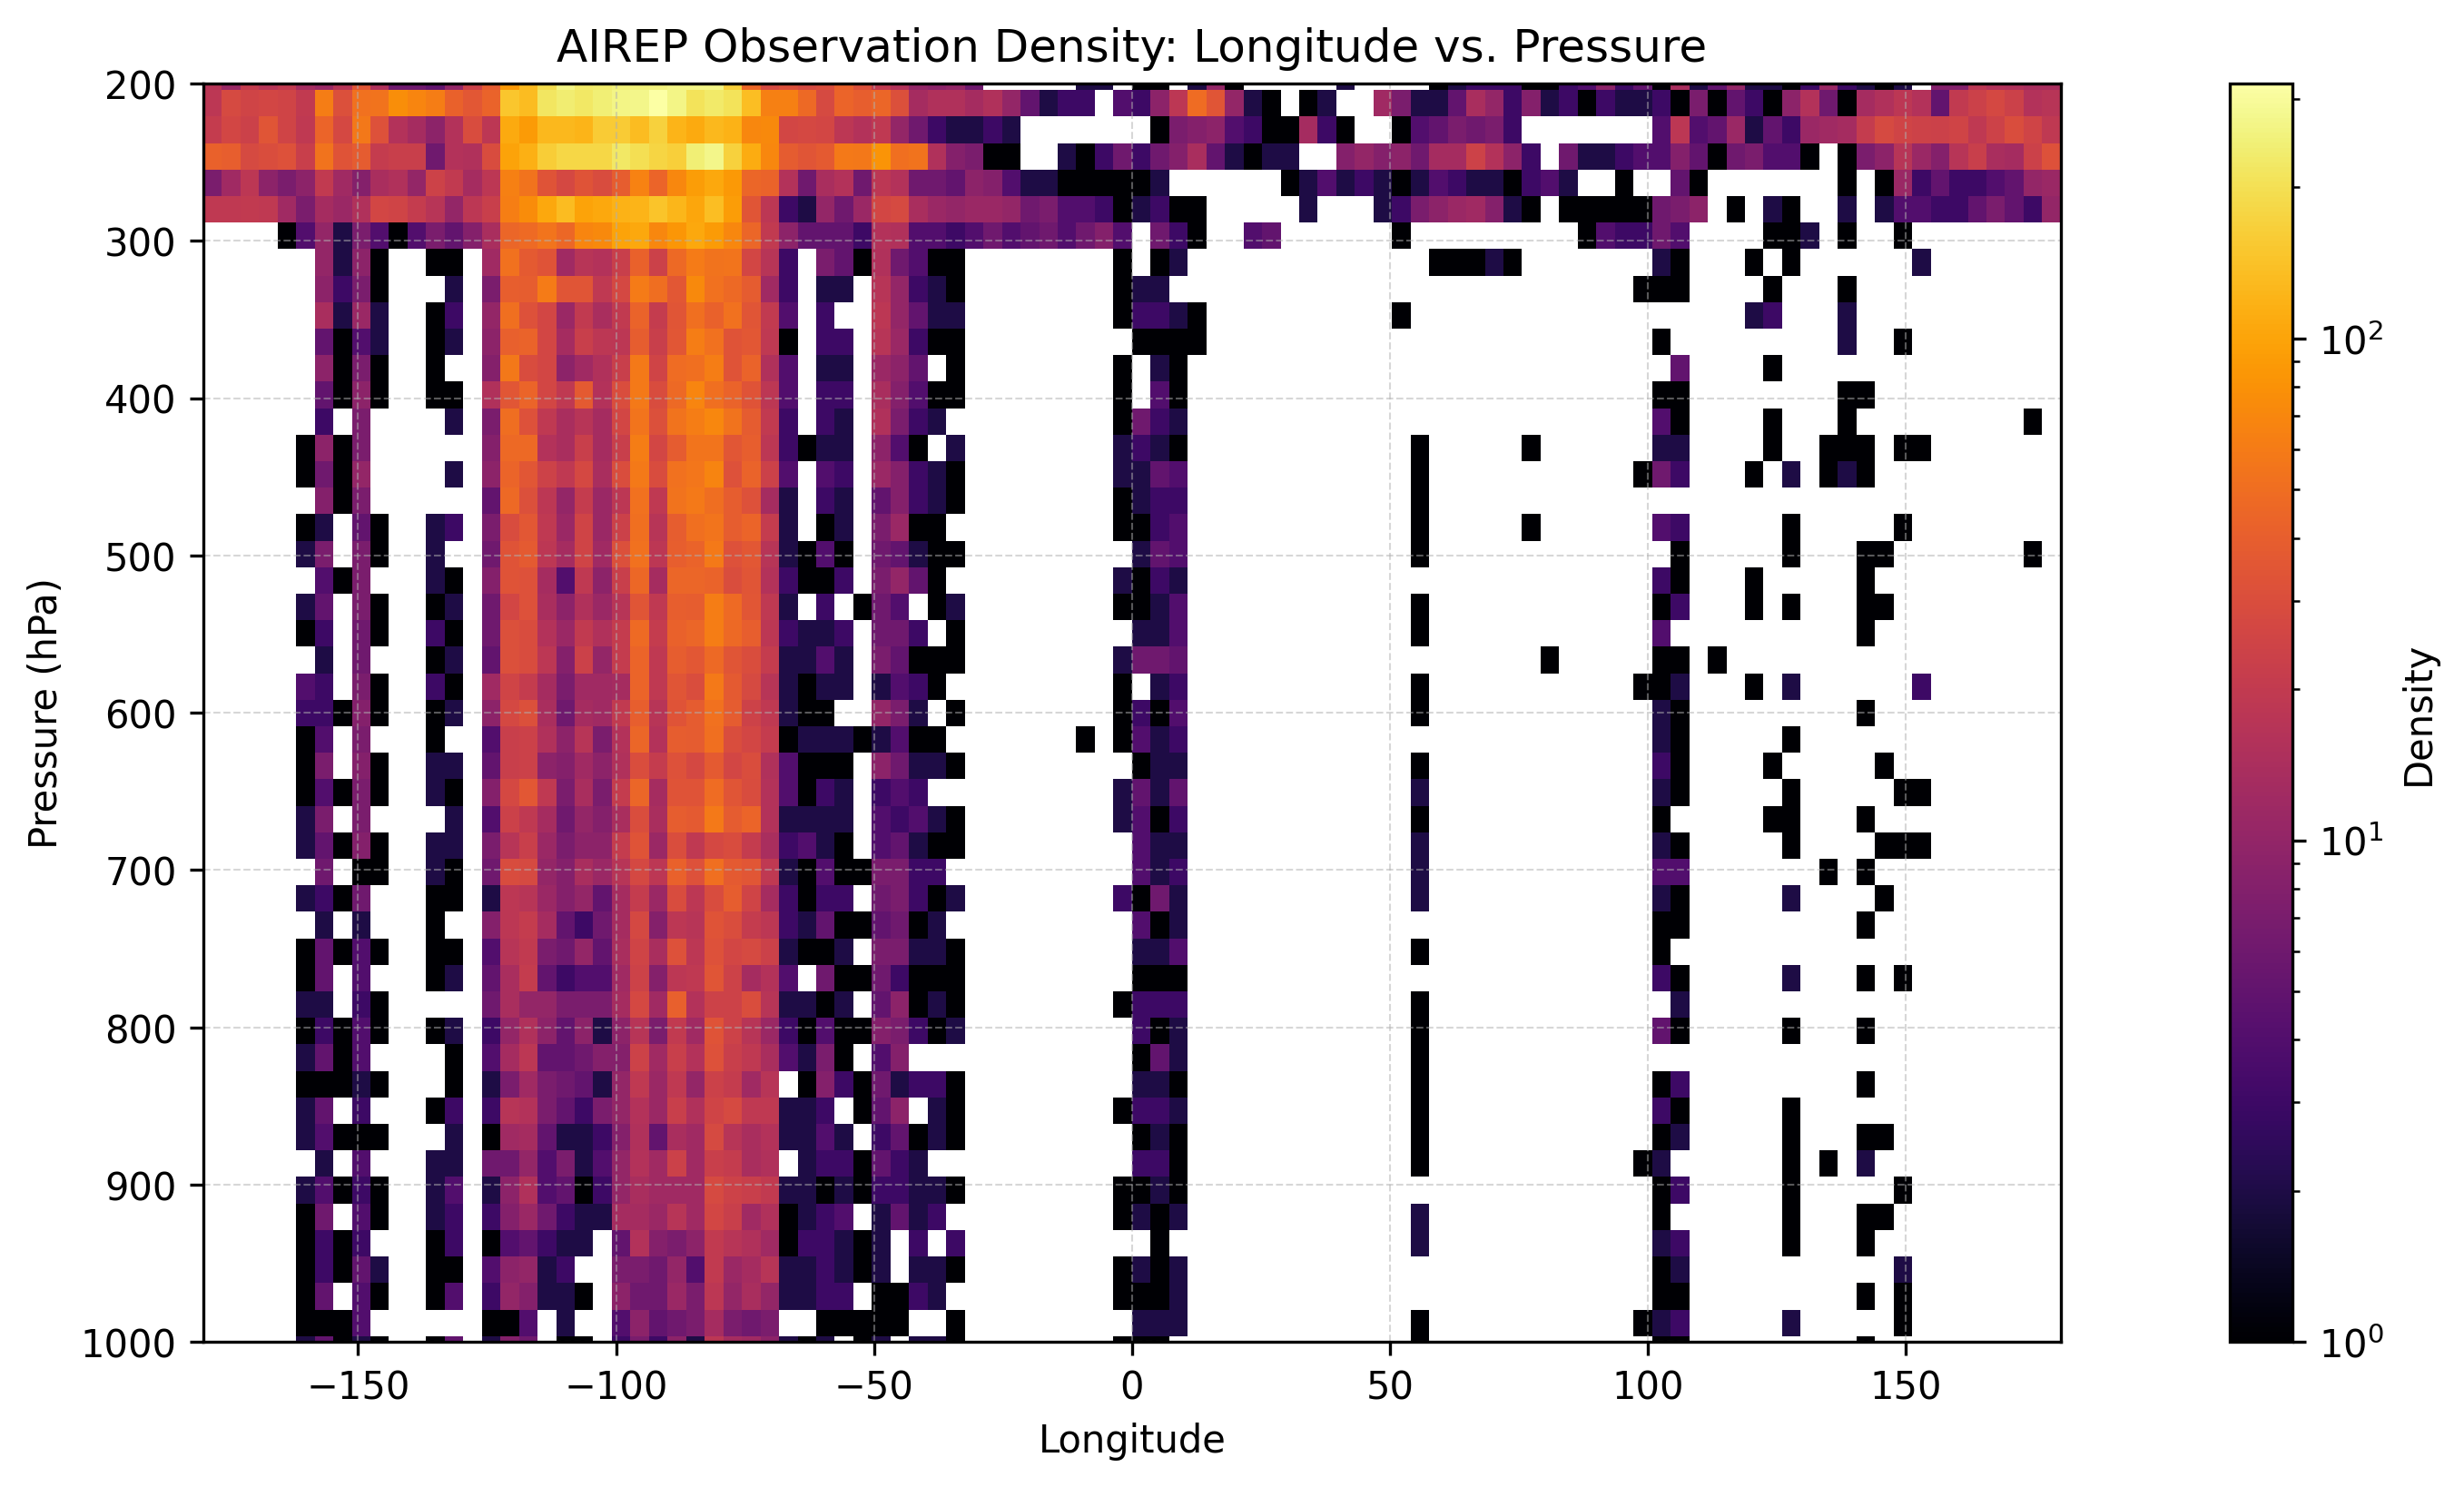
\includegraphics[width=0.9\textwidth]{images/airep_height_density.png}
    \caption{AIREP density vs vertical height in hPa and longitude.}
    \label{fig:airep_plot}
\end{figure}

The following code will generate a density distribution over height and longitudes. 

\begin{codeonly}{Vertical Distribution of AIRPE Observations}
def plot_height_histogram(lons, heights,
                           filename="airep_height_density.png"):
    """Generates a histogram of longitude vs. height, converting pressure
    to altitude with 1000 hPa at the bottom and 200 hPa at the top."""
    fig, ax = plt.subplots(figsize=(10, 6))
    
    # Convert pressure Pa to hPa 
    heights = heights / 100 
    
    # Create 2D histogram
    hist, xedges, yedges = np.histogram2d(lons, heights,
                                          bins=(100, 50))
    
    # Use the same optimized colormap as in global density plot
    pcm = ax.pcolormesh(xedges, yedges, hist.T, cmap='inferno',
                        norm=plt.matplotlib.colors.LogNorm(
                            vmin=hist[hist > 0].min(),
                            vmax=hist.max()))
    
    cbar = fig.colorbar(pcm, ax=ax, orientation='vertical',
                        fraction=0.04, pad=0.08)
    cbar.set_label("Density")
    
    plt.xlabel("Longitude")
    plt.ylabel("Pressure (hPa)")
    plt.title("AIREP Observation Density: Longitude vs. Pressure")
    plt.ylim(1000, 200)  # Invert y-axis so 1000 hPa is at bottom
    plt.grid(True, linestyle='--', linewidth=0.5, alpha=0.5)
    
    plt.savefig(filename, dpi=300, bbox_inches="tight")
    plt.show()
\end{codeonly}



